\documentclass[aspectratio=169]{beamer}

% ========================
% Beamer Theme (gọn, chuyên nghiệp)
% ========================
%\usetheme{Warsaw}
\usetheme{AnnArbor}
\usecolortheme{seahorse}

% ========================
% Import preamble riêng (nếu có)
% ========================

%%%%%%%%%%%%%%%%%%%%%%%%%%%%%%%%%%%%%%%%%%%%%%%%%%%%%%%%%%%%%%%%%%%%%%%
%       BEAMER PREAMBLE - Tối ưu từ Luận văn - XeLaTeX
%%%%%%%%%%%%%%%%%%%%%%%%%%%%%%%%%%%%%%%%%%%%%%%%%%%%%%%%%%%%%%%%%%%%%%%

% --- XeLaTeX và Font ---
\usepackage{fontspec}
\usepackage{pifont}
\usepackage{polyglossia}
\setmainlanguage{vietnamese}
\setotherlanguage{english}

% Cấu hình font (ưu tiên sans-serif cho slide)
\setsansfont{TeX Gyre Heros}[Ligatures=TeX, Scale=1.05] % Font chính cho slide
\setmainfont{Cormorant Garamond}[Ligatures=TeX]         % Font phụ (in ấn)
\setmonofont{Fira Code}[Scale=0.9, Ligatures=TeX]

% Unicode math
\usepackage{unicode-math}
\setmathfont{Latin Modern Math}

% --- Các gói hỗ trợ nội dung ---
\usepackage{xcolor}
\usepackage{minted} % cần compile với -shell-escape
\usepackage{graphicx}
\graphicspath{{images/}} 
\usepackage{amsmath}
\usepackage{tabularx}
\usepackage{tikz}
\usetikzlibrary{positioning, calc, arrows.meta}
\usepackage{pgfplots}
\pgfplotsset{compat=1.18}
\usepackage{hyperref}

% (Tuỳ chọn: chỉ dùng caption nếu cần subfigure)
% \usepackage{caption}
% \usepackage{subcaption}

% Cấu hình màu và minted
\definecolor{darkblue}{RGB}{0,0,139}
\definecolor{lightgray}{gray}{0.95}
\setminted{
    frame=single,
    linenos=true,
    numbersep=10pt,
    bgcolor=lightgray,
    fontsize=\small,
    breaklines=true,
    tabsize=4,
    xleftmargin=10pt,
    escapeinside=||
}

% Cấu hình hyperref
\hypersetup{
    colorlinks=true,
    linkcolor=darkblue,
    urlcolor=darkblue,
    citecolor=darkblue
}

% Macros
\newcommand{\TENLUANVAN}{Hệ thống phát hiện và cảnh báo té ngã thời gian thực tích hợp cảm biến, xử lý ảnh và định vị}
\newcommand{\THESISNAME}{Real-time fall detection and alert system integrating sensors, image processing, and positioning}
\newcommand{\TENTACGIA}{Trần Đức Hảo}
\newcommand{\MASOSV}{1734011}
\newcommand{\BOMON}{Viễn thông}
\newcommand{\TENNGUOIHUONGDAN}{PSG.TS Hà Hoàng Kha}
\newcommand{\NAMBAOVE}{2025}
\newcommand{\KHOA}{Khoa Điện – Điện tử}
\newcommand{\TRUONG}{Trường Đại học BK.HCM}
\newcommand{\DEPARTMENT}{\KHOA}
\newcommand{\TENTACGIAFACULTY}{\TENTACGIA}
\newcommand{\MSSV}{\MASOSV}
\newcommand{\TENCANBO}{\TENNGUOIHUONGDAN}
% --- Metadata Beamer ---
\title[ESP32]{\TENLUANVAN}
\author[Trần Đức Hảo]{\TENTACGIA}
\date{\today}


% ========================
% Metadata
% ========================
\title[Fall Detection System]{\TENLUANVAN}
\author{\TENTACGIA}
\institute{\TRUONG}
\date{\today}

% ========================
% Bắt đầu tài liệu
% ========================
\begin{document}

% --- Title + Outline ---

% --- Slide 1: Trang tiêu đề ---
\begin{frame}
    \titlepage
\end{frame}

% --- Slide 2: Thông tin tác giả & người hướng dẫn ---
\begin{frame}
    \centering
    {\Large \textbf{Tác giả:} \TENTACGIA \par}
    {\Large \textbf{Người hướng dẫn:} \TENNGUOIHUONGDAN \par}
    \vspace{0.5cm}
    {\small Khoa: \KHOA \par}
    {\small Trường: \TRUONG \par}
    \vfill
    {\footnotesize \today}
\end{frame}

% --- Slide  Trang  table of content---
\AtBeginDocument{%
  \begin{frame}{Mục lục}
    \tableofcontents[hideallsubsections]
  \end{frame}
}


% --- Introduction ---

% --- Bắt đầu SECTION: GIỚI THIỆU & BỐI CẢNH ---
\section{I-GIỚI THIỆU}

% --- Slide 3: Vấn đề toàn cầu ---
\begin{frame}{Té ngã: Vấn đề chung toàn cầu}
    \begin{columns}[T]
        \begin{column}{0.48\textwidth}
            \begin{itemize}
                \item Nguyên nhân chính gây chấn thương và tử vong không cố ý.
                \item \textbf{WHO}: $\sim646,000$ ca tử vong/năm; $>80\%$ ở các nước thu nhập trung bình/thấp.
                \item Người cao tuổi: \textbf{30\%} té ngã/năm ở người $>65$ tuổi, tăng lên \textbf{50\%} ở người $>85$ tuổi.
            \end{itemize}
        \end{column}
        \begin{column}{0.48\textwidth}
            \begin{figure}
                \centering
                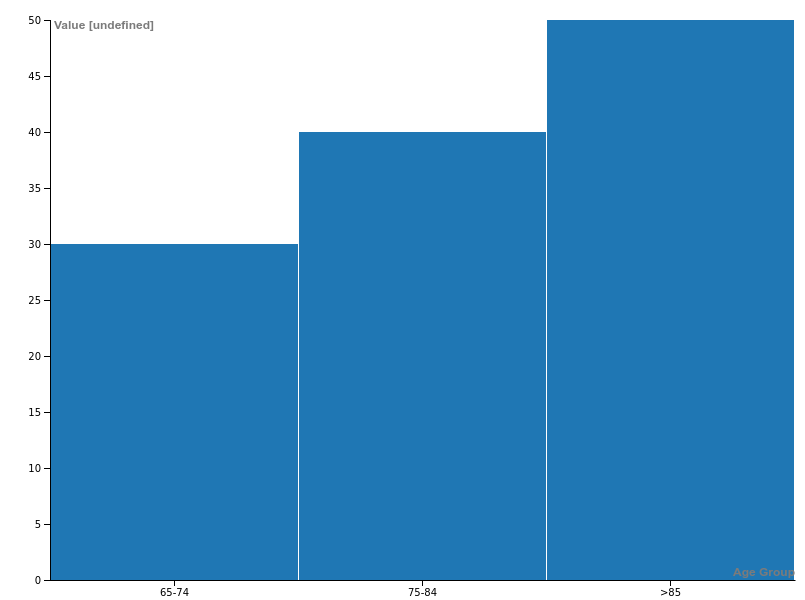
\includegraphics[width=\textwidth]{images/fall_status_who.png}
                \caption{Tỷ lệ té ngã theo nhóm tuổi}
            \end{figure}
        \end{column}
    \end{columns}
\end{frame}




% --- Bắt đầu SUBSECTION: Nghiên cứu liên quan ---
\subsection{Tình hình nghiên cứu}
% --- Slide 5: Nghiên cứu trong và ngoài nước ---
\begin{frame}{Nghiên cứu trong và ngoài nước}
    \begin{columns}[T]
        \begin{column}{0.48\textwidth}
            \textbf{Quốc tế}
            \begin{itemize}
                \item \textbf{Xu hướng}: Sử dụng YOLO, Transformer, AI nhẹ, cảm biến mmWave.
                \item \textbf{Thành tựu}: Giảm false alarm, tối ưu cho thiết bị biên, Sensor Fusion.
            \end{itemize}
        \end{column}
        \begin{column}{0.48\textwidth}
            \textbf{Trong nước}
            \begin{itemize}
                \item \textbf{Thực trạng}: Chủ yếu mô hình thử nghiệm (PoC) với ESP32, Arduino.
                \item \textbf{Hạn chế}: Thiếu dữ liệu lớn, độ chính xác thấp (75-85\%), thiếu tích hợp đa phương thức.
            \end{itemize}
        \end{column}
    \end{columns}
\end{frame}


%% --- Bắt đầu SECTION: THIẾT KẾ & THỰC HIỆN ---
\subsection{MỤC TÊU, NHIỆM VỤ ĐẶT RA THỰC HIỆN ĐỀ TÀI}

% --- Slide 7: Kiến trúc hệ thống tổng thể ---
\begin{frame}{Kiến trúc hệ thống tổng thể}
    \begin{figure}
        \centering
        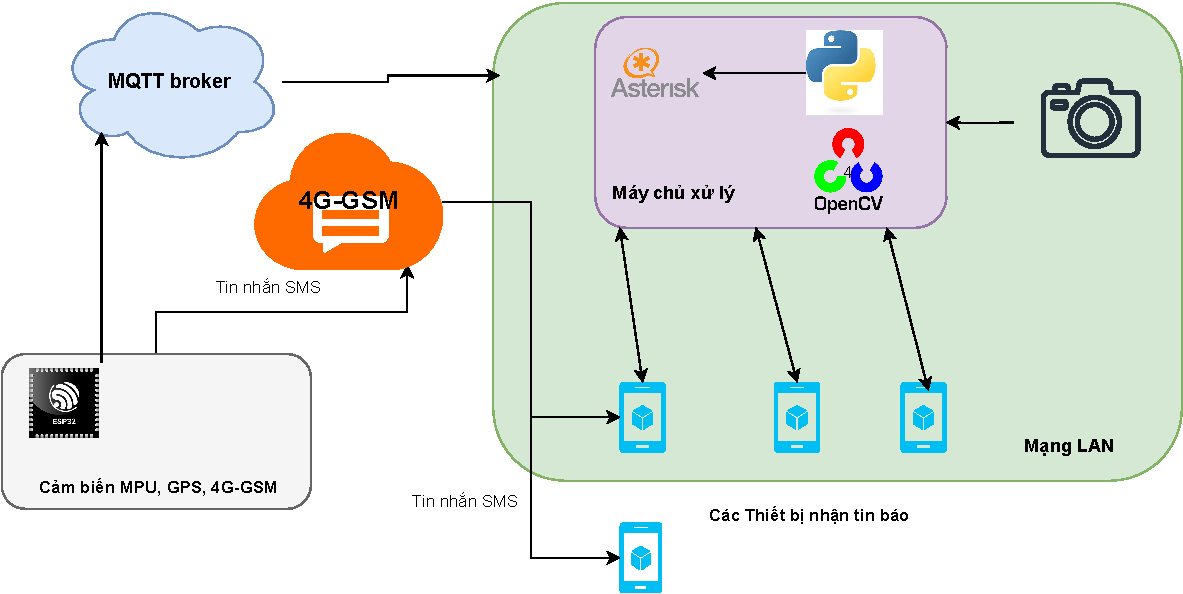
\includegraphics[width=0.8\textwidth]{images/resuilt_structure_diagram.pdf}
        \caption{Sơ đồ hệ thống tổng thể}
    \end{figure}
\end{frame}

% --- Slide 8: Hệ thống nhúng (ESP32) ---
\begin{frame}{Hệ thống nhúng (ESP32)}
    \begin{columns}[T]
        \begin{column}{0.48\textwidth}
            \begin{itemize}
                \item \textbf{Phần cứng}: ESP32, MPU6050, GPS EC800K.
                \item \textbf{Nguyên lý}: Phát hiện té ngã dựa trên ngưỡng động học.
                \item \textbf{Giao tiếp}: Gửi cảnh báo qua \textbf{MQTT và SMS}.
                \item \textbf{Ưu điểm}: Thiết bị độc lập, tiết kiệm năng lượng, dễ mở rộng.
            \end{itemize}
        \end{column}
        \begin{column}{0.48\textwidth}
            \begin{figure}
                \centering
                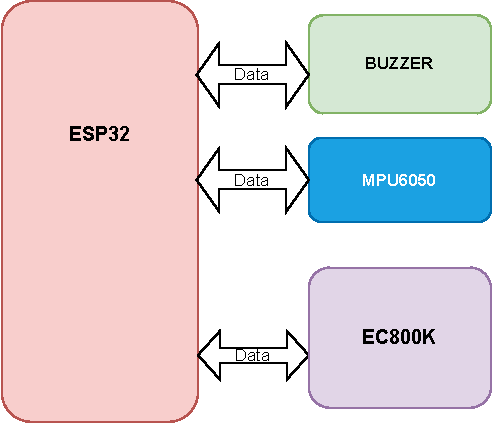
\includegraphics[width=\textwidth]{images/module1_block_diagram-crop.pdf}
                \caption{Sơ đồ nhúng ESP32 \& truyền thông}
            \end{figure}
        \end{column}
    \end{columns}
\end{frame}

% --- Slide 9: Hệ thống phân tích hình ảnh ---
\begin{frame}{Hệ thống phân tích hình ảnh}
    \begin{columns}[T]
        \begin{column}{0.48\textwidth}
            \begin{itemize}
                \item \textbf{Công nghệ}: MediaPipe, OpenCV, YOLO để trích xuất các điểm khớp xương (keypoints) và phân tích tư thế.
                \item \textbf{Quy trình}: Phân tích góc nghiêng, vận tốc, tỉ lệ khung xương để nhận diện té ngã.
                \item \textbf{Thuật toán}: Sử dụng các mô hình học máy (ML) như SVM, Decision Tree.
            \end{itemize}
        \end{column}
        \begin{column}{0.48\textwidth}
            \begin{figure}
                \centering
                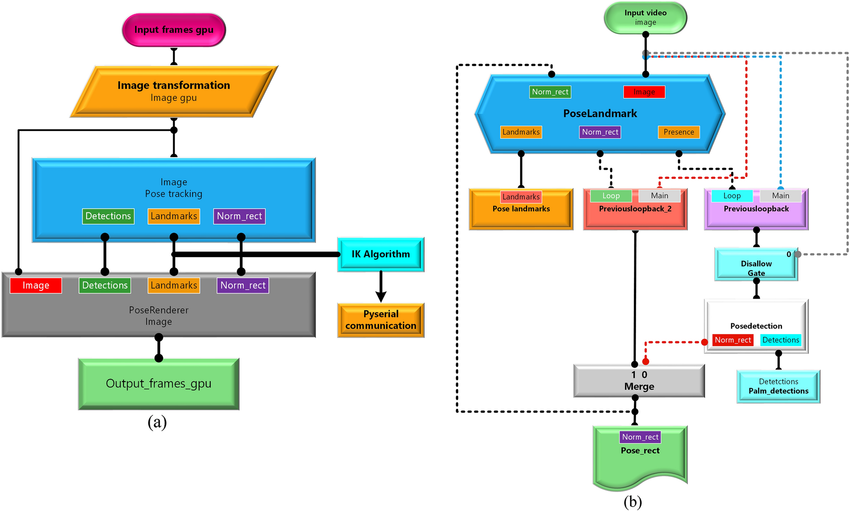
\includegraphics[width=\textwidth]{images/media_pose_pipeline.png}
                \caption{Pipeline MediaPipe + YOLO}
            \end{figure}
        \end{column}
    \end{columns}
\end{frame}



\section{Kết quả và Đánh giá}
% --- Slide 10: Hiệu năng và giới hạn ---
\begin{frame}{Hiệu năng và Giới hạn}
    \begin{columns}[T]
        \begin{column}{0.48\textwidth}
            \textbf{Mục tiêu Hiệu năng}
            \begin{itemize}
                \item Tổng độ trễ $<5$ giây.
                \item Độ chính xác $>90\%$, False Alarm $<8\%$.
                \item Uptime dịch vụ MQTT $>99\%$.
            \end{itemize}
        \end{column}
        \begin{column}{0.48\textwidth}
            \textbf{Giới hạn nghiên cứu}
            \begin{itemize}
                \item Hoạt động trong nhà với điều kiện ánh sáng và mạng ổn định.
                \item Nguyên mẫu \textbf{ESP32} chưa tích hợp học sâu toàn phần.
                \item Không phát triển app di động/web phức tạp.
            \end{itemize}
        \end{column}
    \end{columns}
\end{frame}

%% slides/01_introduction/05_introsummary.tex
\subsection{Tóm tắt Chương}
\label{sec:chapter1_conclusion}

\begin{frame}{Tóm tắt Giới thiệu}
\begin{table}
\centering
\footnotesize
\begin{tabular}{@{}lp{0.8\textwidth}@{}}
\toprule
\textbf{Nội dung} & \textbf{Mô tả} \\
\midrule
Tổng quan & \TENLUANVAN: Giải pháp giám sát sức khỏe chủ động cho người cao tuổi và bệnh nhân, tích hợp \textbf{IMU} và \textbf{Thị giác Máy tính (CV)}. \\
Khoảng trống kỹ thuật & Thiếu giải pháp tích hợp \textbf{Human Pose Estimation} (MediaPipe Pose) với phần cứng nhúng chi phí thấp (\textbf{ESP32}). Kết hợp \textbf{độ chính xác cao} (CV) và \textbf{tính di động, tiết kiệm} (IMU). \\
Mục tiêu nghiên cứu & Xây dựng hệ thống phát hiện té ngã \textbf{đáng tin cậy}, \textbf{hiệu quả}, phân tích sự kiện đa giai đoạn với dữ liệu \textbf{đa cảm biến}. \\
Tiếp theo & Chương \textit{Cơ sở Lý thuyết}: Nguyên lý \textbf{CV}, \textbf{HPE}, \textbf{Hệ thống nhúng} cho thiết kế giải pháp. \\
\bottomrule
\end{tabular}
\end{table}
\end{frame}


% --- Background ---
\begin{frame}{Tổng quan các phương pháp phát hiện té ngã}
\scriptsize
\begin{tabular}{|p{0.18\linewidth}|p{0.22\linewidth}|p{0.25\linewidth}|p{0.25\linewidth}|}
\hline
\textbf{Phương pháp} & \textbf{Cơ chế} & \textbf{Ưu điểm} & \textbf{Nhược điểm} \\
\hline
Đeo được & IMU (gia tốc kế, con quay hồi chuyển); phát hiện gia tốc/tư thế bất thường & Phản hồi nhanh; chính xác; chi phí thấp & Cần đeo liên tục; dễ false positive; pin/hiệu chuẩn \\
\hline
Môi trường & Cảm biến cố định: sàn áp suất, PIR, âm thanh; AI phân tích & Không xâm phạm; giám sát nhiều người; tích hợp smart home & Chi phí cao; phạm vi hạn chế; nhầm vật thể \\
\hline
Thị giác & Camera RGB/RGB-D/IR; pose estimation (OpenPose/MediaPipe) & Thông tin trực quan; không cần đeo; tích hợp giám sát & Quyền riêng tư; phụ thuộc ánh sáng; cần phần cứng mạnh \\
\hline
Đa phương thức & Kết hợp IMU + camera + môi trường; data fusion (Kalman/Deep Learning) & Độ chính xác cao; giảm cảnh báo sai; mở rộng phạm vi; kinh tế & Phức tạp; tốn năng lượng; đồng bộ khó \\
\hline
\end{tabular}

\vspace{0.3em}
\begin{itemize}\scriptsize
    \item Kết hợp dữ liệu để xác nhận té ngã, giảm false positive.  
    \item Chế độ linh hoạt: In-situ (cục bộ) + Mobile (edge device).  
    \item Bảo mật: xử lý cục bộ, chỉ gửi dữ liệu tối thiểu, tùy chỉnh khu vực nhạy cảm.
\end{itemize}
\end{frame}



% Slide 1: Tổng quan
\begin{frame}
\frametitle{Các Giao Thức Truyền Thông trong Hệ Thống Cảnh Báo IoT}
\begin{center}
\Large Hệ thống phát hiện ngã với ba giao thức cốt lõi
\end{center}

\begin{itemize}
\item \textbf{SIP}: Truyền tải âm thanh/video cảnh báo thời gian thực
\item \textbf{MQTT}: Vận chuyển dữ liệu cảm biến từ thiết bị IoT  
\item \textbf{JSON}: Định dạng cấu trúc dữ liệu trao đổi
\end{itemize}

\begin{block}{Mục tiêu}
Xây dựng hệ thống cảnh báo không gián đoạn, độ trễ thấp từ cảm biến đến cuộc gọi VoIP
\end{block}
\end{frame}

% SIP
\begin{frame}
\frametitle{Giao thức SIP - Khởi tạo Phiên}
\textbf{Chức năng chính:}
\begin{itemize}
\item Thiết lập cuộc gọi VoIP từ hệ thống cảnh báo
\item Kết nối với Asterisk PBX để gọi điện thoại
\item Truyền âm thanh cảnh báo qua RTP
\end{itemize}
\textbf{Các bước hoạt động:}
\begin{enumerate}
\item REGISTER: Đăng ký thiết bị với server
\item INVITE: Khởi tạo cuộc gọi cảnh báo
\item ACK: Xác nhận kết nối thành công
\item RTP: Truyền dữ liệu âm thanh
\item BYE: Kết thúc cuộc gọi
\end{enumerate}
\begin{alertblock}{Lưu ý}
Sử dụng ICE để xuyên NAT, TLS/SRTP để bảo mật
\end{alertblock}
\end{frame}

\begin{frame}
\frametitle{Phân biệt Đường tín hiệu và Đường truyền phương tiện}

\begin{block}{Đường tín hiệu (Signaling Path)}
\begin{itemize}
\item Mang các tin nhắn SIP (INVITE, BYE, 200 OK, v.v.)
\item Thiết lập, quản lý và kết thúc cuộc gọi
\item Sử dụng TCP hoặc UDP
\end{itemize}
\end{block}

\begin{block}{Đường truyền phương tiện (Media Path)}
\begin{itemize}
\item Mang dữ liệu thoại/video thực tế
\item Sử dụng RTP qua UDP
\item Truyền trực tiếp giữa các điểm cuối
\end{itemize}
\end{block}

\end{frame}

\begin{frame}
\frametitle{Sơ đồ Đường tín hiệu và Đường truyền phương tiện}

\begin{figure}[h]
\centering
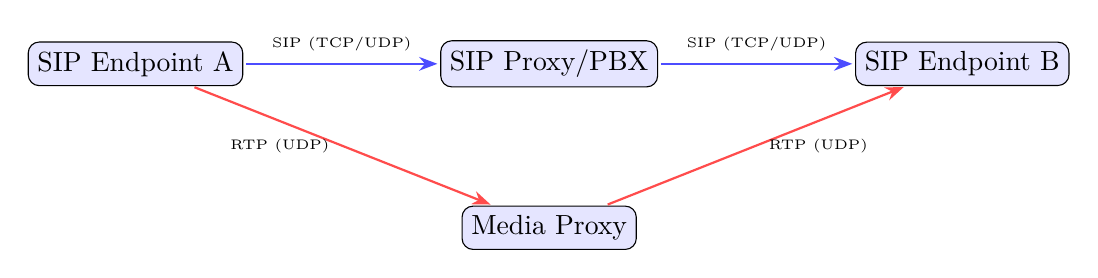
\begin{tikzpicture}[
    box/.style={rectangle, draw, rounded corners, minimum height=1em, minimum width=2.5em, align=center, fill=blue!10}, 
    signal_arrow/.style={-Stealth, thick, blue!70!white, shorten >=1pt, shorten <=1pt}, 
    media_arrow/.style={-Stealth, thick, red!70!white, shorten >=1pt, shorten <=1pt}, 
    label_style/.style={font=\tiny, align=center, text=black},
    node distance=1.8cm and 2.5cm 
]
    % Các Node
    \node[box] (A) {SIP Endpoint A};
    \node[box, right=of A] (Proxy) {SIP Proxy/PBX}; 
    \node[box, right=of Proxy] (B) {SIP Endpoint B};
    \node[box, below=1.5cm of Proxy] (MediaProxy) {Media Proxy}; 
    
    % Đường tín hiệu
    \draw[signal_arrow] (A) -- node[above=1pt, label_style] {SIP (TCP/UDP)} (Proxy);
    \draw[signal_arrow] (Proxy) -- node[above=1pt, label_style] {SIP (TCP/UDP)} (B);
    
    % Đường truyền phương tiện
    \draw[media_arrow] (A) -- node[midway, left=1pt, label_style] {RTP (UDP)} (MediaProxy); 
    \draw[media_arrow] (MediaProxy) -- node[midway, right=1pt, label_style] {RTP (UDP)} (B); 
\end{tikzpicture}
\end{figure}

\end{frame}

\begin{frame}
\frametitle{Giao thức ICE (Interactive Connectivity Establishment)}

\begin{block}{Vấn đề}
Các thiết bị thường nằm sau NAT/firewall, ngăn cản truyền dữ liệu RTP trực tiếp
\end{block}

\begin{block}{Giải pháp ICE}
\begin{itemize}
\item \textbf{Local IP:} Địa chỉ IP nội bộ của thiết bị
\item \textbf{STUN:} Phát hiện địa chỉ IP công cộng và cổng NAT
\item \textbf{TURN:} Máy chủ chuyển tiếp khi STUN thất bại
\end{itemize}
\end{block}

\begin{alertblock}{Lưu ý}
Quá trình ICE thực hiện qua SDP trong thông điệp SIP
\end{alertblock}

\end{frame}

\begin{frame}
\frametitle{SIP trong Hệ Thống Cảnh Báo Asterisk}

\begin{block}{Lợi ích}
\begin{itemize}
\item \textbf{Quản lý tập trung:} Đồng nhất cấu hình và quản lý thiết bị
\item \textbf{Tương thích cao:} Hỗ trợ đa dạng nền tảng và thiết bị
\item \textbf{Chuẩn mở:} Tích hợp dễ dàng với hạ tầng hiện có
\item \textbf{Bảo mật:} Hỗ trợ TLS (SIP) và SRTP (RTP)
\end{itemize}
\end{block}

\begin{block}{Vai trò của Asterisk}
Đóng vai trò như SIP server, xử lý đăng ký và định tuyến cuộc gọi
\end{block}

\end{frame}

\begin{frame}
\frametitle{Luồng Phân Phối Cảnh Báo (1/2)}

\begin{block}{1. Đăng ký}
\begin{itemize}
\item Thiết bị SIP gửi REGISTER tới Asterisk
\item Xác thực qua username/password trong header Authorization
\end{itemize}
\end{block}

\begin{block}{2. Thiết lập phiên}
\begin{itemize}
\item Ứng dụng Linux ra lệnh \texttt{Originate} qua AMI
\item Asterisk gửi INVITE → 180 Ringing → 200 OK → ACK
\item Sử dụng header \texttt{Alert-Info: ;info=alert-autoanswer}
\end{itemize}
\end{block}

\end{frame}

\begin{frame}
\frametitle{Luồng Phân Phối Cảnh Báo (2/2)}

\begin{block}{3. Trao đổi dữ liệu}
\begin{itemize}
\item Dữ liệu cảnh báo truyền qua RTP
\item TTS (Text-to-Speech) tạo âm thanh từ văn bản
\item Sử dụng codec G.711 hoặc G.729
\end{itemize}
\end{block}

\begin{block}{4. Kết thúc phiên}
\begin{itemize}
\item Một bên gửi BYE
\item Bên kia phản hồi 200 OK
\end{itemize}
\end{block}

\end{frame}

\begin{frame}
\frametitle{Tích Hợp SMS qua SIP}

\begin{block}{Cấu hình}
\begin{itemize}
\item Kích hoạt \texttt{textsupport=yes} trong \texttt{sip.conf}
\item Định nghĩa logic xử lý trong \texttt{extensions.conf}
\end{itemize}
\end{block}

\begin{block}{Thực hiện}
\begin{itemize}
\item Sử dụng lệnh \texttt{MessageSend}
\item Gửi tin nhắn SIP MESSAGE
\item Tích hợp SMS gateway để chuyển tiếp sang mạng di động
\end{itemize}
\end{block}

\end{frame}

% Slide 3: Giao thức MQTT
\begin{frame}
\frametitle{Giao thức MQTT - Tổng quan}

\begin{block}{Định nghĩa}
\begin{itemize}
\item MQTT = Message Queuing Telemetry Transport
\item Giao thức nhẹ, tối ưu cho IoT và M2M
\item Hoạt động trên TCP/IP với cơ chế kết nối lâu dài
\end{itemize}
\end{block}

\begin{block}{Đặc điểm}
\begin{itemize}
\item Thiết kế cho thiết bị có tài nguyên hạn chế
\item Phù hợp với băng thông thấp
\item Hỗ trợ kết nối không ổn định
\item Tiêu chuẩn OASIS cho IoT messaging
\end{itemize}
\end{block}

\end{frame}

\begin{frame}
\frametitle{Kiến trúc Publish/Subscribe của MQTT}

\begin{figure}[h]
\centering
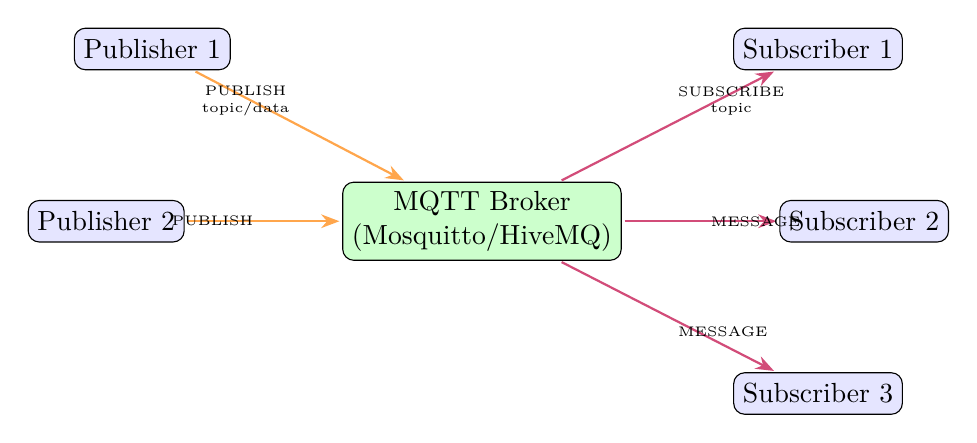
\begin{tikzpicture}[
    broker/.style={rectangle, draw, rounded corners, minimum height=2em, minimum width=3em, align=center, fill=green!20}, 
    client/.style={rectangle, draw, rounded corners, minimum height=1.5em, minimum width=2.5em, align=center, fill=blue!10}, 
    pub_arrow/.style={-Stealth, thick, orange!70!white, shorten >=1pt, shorten <=1pt}, 
    sub_arrow/.style={-Stealth, thick, purple!70!white, shorten >=1pt, shorten <=1pt}, 
    label_style/.style={font=\tiny, align=center, text=black},
    node distance=2cm
]
    % Broker trung tâm
    \node[broker] (broker) {MQTT Broker \\ (Mosquitto/HiveMQ)};
    
    % Publishers
    \node[client, above left=of broker] (pub1) {Publisher 1};
    \node[client, left=of broker] (pub2) {Publisher 2};
    
    % Subscribers
    \node[client, above right=of broker] (sub1) {Subscriber 1};
    \node[client, right=of broker] (sub2) {Subscriber 2};
    \node[client, below right=of broker] (sub3) {Subscriber 3};
    
    % Publish arrows
    \draw[pub_arrow] (pub1) -- node[above left, label_style] {PUBLISH \\ topic/data} (broker);
    \draw[pub_arrow] (pub2) -- node[left, label_style] {PUBLISH} (broker);
    
    % Subscribe arrows
    \draw[sub_arrow] (broker) -- node[above right, label_style] {SUBSCRIBE \\ topic} (sub1);
    \draw[sub_arrow] (broker) -- node[right, label_style] {MESSAGE} (sub2);
    \draw[sub_arrow] (broker) -- node[below right, label_style] {MESSAGE} (sub3);
\end{tikzpicture}
\end{figure}

\end{frame}

\begin{frame}
\frametitle{Lợi ích của mô hình Publish/Subscribe}

\begin{block}{Tách rời không gian (Space Decoupling)}
\begin{itemize}
\item Publisher và Subscriber không cần biết địa chỉ IP của nhau
\item Giao tiếp thông qua broker trung tâm
\end{itemize}
\end{block}

\begin{block}{Tách rời thời gian (Time Decoupling)}
\begin{itemize}
\item Không yêu cầu kết nối đồng thời
\item Hỗ trợ \textbf{retained messages} cho subscriber mới
\item Quản lý \textbf{clean session} cho trạng thái client
\end{itemize}
\end{block}

\begin{block}{Tách rời đồng bộ (Synchronization Decoupling)}
\begin{itemize}
\item Truyền và nhận hoạt động độc lập
\item Giảm độ trễ và tăng hiệu suất
\end{itemize}
\end{block}

\end{frame}


\begin{frame}
\frametitle{Quality of Service (QoS)}

\begin{block}{QoS 0 - At most once}
\begin{itemize}
\item "Fire and forget" - không có xác nhận
\item Nhanh nhất nhưng có thể mất message
\item Phù hợp cho dữ liệu cảm biến thường xuyên
\end{itemize}
\end{block}

\begin{block}{QoS 1 - At least once}
\begin{itemize}
\item Đảm bảo message được gửi ít nhất một lần
\item Có thể trùng lặp message
\item Cân bằng giữa độ tin cậy và hiệu suất
\end{itemize}
\end{block}

\begin{block}{QoS 2 - Exactly once}
\begin{itemize}
\item Đảm bảo message được gửi đúng một lần
\item Chậm nhất nhưng tin cậy nhất
\item Sử dụng cho dữ liệu quan trọng
\end{itemize}
\end{block}

\end{frame}


\begin{frame}
\frametitle{Bảo mật trong MQTT}

\begin{block}{Mã hóa Transport Layer}
\begin{itemize}
\item Hỗ trợ TLS/SSL cho kết nối bảo mật
\item MQTT over TLS (port 8883)
\item Bảo vệ dữ liệu trong quá trình truyền
\end{itemize}
\end{block}

\begin{block}{Xác thực và Ủy quyền}
\begin{itemize}
\item Username/Password authentication
\item Client certificates cho xác thực mạnh
\item Access Control Lists (ACL) kiểm soát quyền truy cập topic
\end{itemize}
\end{block}
\end{frame}

\begin{frame}
\frametitle{Các lệnh MQTT chính}

\begin{block}{Connection Management}
\begin{itemize}
\item \texttt{CONNECT}: Khởi tạo kết nối với broker
\item \texttt{CONNACK}: Xác nhận kết nối từ broker
\item \texttt{DISCONNECT}: Ngắt kết nối một cách graceful
\end{itemize}
\end{block}

\begin{block}{Messaging Operations}
\begin{itemize}
\item \texttt{PUBLISH}: Gửi message tới topic
\item \texttt{PUBACK/PUBREC/PUBREL/PUBCOMP}: QoS acknowledgments
\item \texttt{SUBSCRIBE}: Đăng ký nhận messages từ topic
\item \texttt{SUBACK}: Xác nhận subscription
\item \texttt{UNSUBSCRIBE}: Hủy đăng ký topic
\end{itemize}
\end{block}

\begin{block}{Keep Alive}
\begin{itemize}
\item \texttt{PINGREQ/PINGRESP}: Duy trì kết nối
\end{itemize}
\end{block}

\end{frame}

\begin{frame}
\frametitle{MQTT trong Hệ thống IoT và Cảnh báo}

\begin{block}{Ứng dụng trong IoT}
\begin{itemize}
\item Thu thập dữ liệu từ sensors
\item Điều khiển thiết bị từ xa
\item Giám sát trạng thái hệ thống
\item Gửi thông báo và cảnh báo
\end{itemize}
\end{block}

\begin{block}{Lợi ích cho hệ thống cảnh báo}
\begin{itemize}
\item Kết nối đáng tin cậy với thiết bị IoT
\item Truyền dữ liệu real-time
\item Hỗ trợ offline messaging
\item Scale tốt với nhiều thiết bị
\end{itemize}
\end{block}

\end{frame}

\begin{frame}
\frametitle{Giao thức MQTT - Truyền Dữ Liệu Cảm Biến}

\textbf{Đặc điểm:}
\begin{itemize}
\item Nhẹ, tiết kiệm băng thông cho thiết bị IoT
\item Mô hình Publish/Subscribe qua Broker
\item Hỗ trợ 3 mức QoS đảm bảo độ tin cậy
\end{itemize}

\textbf{Mức QoS:}
\begin{itemize}
\item \textcolor{green}{\textbf{QoS 0}}: Gửi một lần (dữ liệu thường)
\item \textcolor{orange}{\textbf{QoS 1}}: Ít nhất một lần (có xác nhận)
\item \textcolor{red}{\textbf{QoS 2}}: Đúng một lần (cảnh báo quan trọng)
\end{itemize}

\textbf{Ví dụ topic:} \texttt{sensor/room/temperature}, \texttt{alert/fall/detected}
\end{frame}

%----------------------JSON--------------------%
% slides/02_background/07_background_json.tex

\begin{frame}
\frametitle{JSON - JavaScript Object Notation}
\begin{block}{Định nghĩa}
\begin{itemize}
\item JSON: JavaScript Object Notation.
\item Định dạng dữ liệu nhẹ, dễ đọc, dùng để trao đổi dữ liệu.
\item Độc lập với ngôn ngữ, dựa trên cú pháp JavaScript.
\end{itemize}
\end{block}

\begin{block}{Đặc điểm}
\begin{itemize}
\item Định dạng dễ đọc, dùng cho lưu trữ và truyền dữ liệu.
\item Cấu trúc gồm cặp \texttt{key:value}, dùng \texttt{\{\}}.
\item Chuẩn phổ biến trong ứng dụng IoT.
\end{itemize}
\end{block}

\begin{block}{Tiêu chuẩn}
RFC 8259: Chuẩn Internet cho định dạng trao đổi dữ liệu JSON.
\end{block}
\end{frame}

\begin{frame}[fragile]
\frametitle{Cấu trúc JSON cơ bản}
\begin{block}{Cấu trúc dữ liệu}
\begin{itemize}
\item \textbf{Object}: \texttt{\{key: value\}}
\item \textbf{Array}: \texttt{[value1, value2]}
\item \textbf{Kiểu giá trị}: String, Number, Boolean, null, Object, Array.
\end{itemize}
\end{block}

\begin{exampleblock}{Ví dụ JSON}
\begin{minted}[frame=single, linenos, breaklines, fontsize=\footnotesize]{json}
{
  "device_id": "ESP32_001",
  "temperature": 25.5,
  "sensors": ["temp", "light"]
}
\end{minted}
\end{exampleblock}
\end{frame}

\begin{frame}
\frametitle{Ứng dụng JSON trong IoT}
\begin{block}{Lưu cấu hình}
\begin{itemize}
\item Cấu hình thiết bị IoT (Wi-Fi, MQTT).
\item Lưu thông số cảm biến và máy chủ.
\end{itemize}
\end{block}

\begin{block}{Trao đổi dữ liệu}
\begin{itemize}
\item Định dạng payload cho MQTT, API.
\item Gửi thông báo cảnh báo trong hệ thống.
\end{itemize}
\end{block}

\begin{block}{Lợi ích}
\begin{itemize}
\item Tự mô tả, nhẹ hơn XML.
\item Tương thích đa nền tảng.
\end{itemize}
\end{block}
\end{frame}

\begin{frame}[fragile]
\frametitle{Ví dụ: Cấu hình ESP32}
\begin{minted}[frame=single, linenos, breaklines, fontsize=\footnotesize]{json}
{
  "network": {
    "ssid": "IoT_Network",
    "mqtt_broker": "192.168.1.100"
  },
  "device": {
    "id": "ESP32_001",
    "update_interval": 30
  }
}
\end{minted}
\end{frame}

\begin{frame}
\frametitle{Thư viện JSON cho hệ thống nhúng}

\begin{block}{json-c}
\begin{itemize}
\item Thư viện JSON cho C/C++.
\item Hỗ trợ phân tích cú pháp, tạo JSON.
\end{itemize}
\end{block}

\begin{block}{FirebaseJson}
\begin{itemize}
\item Thư viện dễ dùng, hỗ trợ JSON phức tạp.
\item Dựa trên cJSON, phù hợp IoT.
\end{itemize}
\end{block}
\end{frame}



\begin{frame}
\frametitle{JSON trong MQTT và SIP}
\begin{block}{JSON với MQTT}
\begin{itemize}
\item Payload JSON trong topic \texttt{sensor/data}.
\item Lưu cấu hình trong retained messages.
\end{itemize}
\end{block}

\begin{block}{JSON với SIP}
\begin{itemize}
\item Dữ liệu JSON trong custom headers, SIP MESSAGE.
\item Lưu cấu hình ứng dụng SIP.
\end{itemize}
\end{block}

\begin{alertblock}{Lưu ý}
JSON đảm bảo tương tác giữa các giao thức trong hệ sinh thái IoT.
\end{alertblock}
\end{frame}


% Slide 4: JSON và Tích hợp Hệ thống
\begin{frame}
\frametitle{JSON và Tích Hợp Hệ Thống}

\textbf{JSON - Định dạng dữ liệu:}
\begin{itemize}
\item Nhẹ, dễ đọc, tương thích đa nền tảng
\item Cấu hình thiết bị và trao đổi dữ liệu cảm biến
\item Tối ưu payload cho MQTT
\end{itemize}

\textbf{Luồng tích hợp hoàn chỉnh:}
\begin{enumerate}
\item ESP32 phát hiện ngã → tạo JSON payload
\item Gửi qua MQTT topic với QoS phù hợp  
\item Ứng dụng trung gian nhận và xử lý JSON
\item Kích hoạt cuộc gọi SIP qua Asterisk AMI
\item Phát cảnh báo âm thanh đến điện thoại
\end{enumerate}
\end{frame}

% Slide 5: Kết luận và Tối ưu
\begin{frame}
\frametitle{Kết Luận và Tối Ưu Hóa kết hợp cá phương thức}

\textbf{Lợi ích của việc kết hợp 3 giao thức:}
\begin{itemize}
\item \textbf{MQTT}: Thu thập dữ liệu hiệu quả từ cảm biến
\item \textbf{JSON}: Cấu trúc dữ liệu linh hoạt, dễ xử lý
\item \textbf{SIP}: Cảnh báo âm thanh tức thì, đáng tin cậy
\end{itemize}

\textbf{Các biện pháp tối ưu:}
\begin{itemize}
\item Payload JSON nhỏ gọn tiết kiệm năng lượng
\item QoS MQTT phù hợp với mức độ quan trọng
\item Tự động kết nối lại khi mất kết nối
\item Bảo mật TLS cho MQTT và SIP
\end{itemize}

\begin{block}{Kết quả}
Hệ thống cảnh báo tự động, tin cậy từ thiết bị nhúng đến cuộc gọi VoIP
\end{block}
\end{frame}


\subsection{CƠ SỞ LÝ THUYẾT VỀ THỊ GIÁC MÁY TÍNH (CV)}
\begin{frame}
\frametitle{Định nghĩa và Mục tiêu}
\begin{block}{Định nghĩa}
\textbf{Thị giác Máy tính (CV)}: Lĩnh vực AI cho phép máy tính xử lý, phân tích và diễn giải hình ảnh/video, mô phỏng thị giác con người.
\end{block}

\begin{block}{Mục tiêu}
\begin{itemize}
\item Tái tạo khả năng nhận thức thị giác với tốc độ, độ chính xác và quy mô vượt trội.
\item Ứng dụng trong \TENLUANVAN, đặc biệt là \textbf{Ước lượng Tư thế Người (HPE)}.
\end{itemize}
\end{block}
\end{frame}

\begin{frame}
\frametitle{Pipeline Cơ bản của Hệ thống CV}
\begin{block}{Quy trình}
\begin{enumerate}
\item \textbf{Thu nhận dữ liệu}: Thu thập ảnh/video từ camera.
\item \textbf{Tiền xử lý}: Chuẩn hóa kích thước, điều chỉnh sáng/tương phản, giảm nhiễu.
\item \textbf{Trích xuất đặc trưng}: Chuyển pixel thành đặc trưng trừu tượng (cạnh, góc, kết cấu).
\item \textbf{Phân tích và quyết định}: Phân loại, nhận dạng hoặc ước lượng tư thế.
\end{enumerate}
\end{block}

\begin{exampleblock}{Minh họa}
\begin{center}
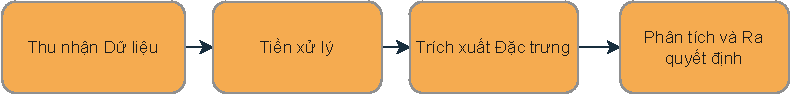
\includegraphics[width=0.9\textwidth]{images/vision_flow-crop.pdf}
\caption{Quy trình tổng thể của hệ thống CV.}
\label{fig:cv_pipeline}
\end{center}
\end{exampleblock}
\end{frame}

\begin{frame}
\frametitle{Phân loại Bài toán CV}
\begin{block}{Các bài toán cốt lõi}
\begin{itemize}
\item \textbf{Phân loại Ảnh}: Gán nhãn cho toàn bộ ảnh (VD: "Người", "Xe").
\item \textbf{Phát hiện Đối tượng}: Xác định vị trí và nhãn bằng hộp giới hạn.
\item \textbf{Phân đoạn Ảnh}:
\begin{itemize}
\item \textbf{Ngữ nghĩa}: Gán nhãn từng pixel (VD: Đường, Cây).
\item \textbf{Thể hiện}: Phân biệt các cá thể cùng lớp.
\end{itemize}
\item \textbf{Ước lượng Tư thế Người (HPE)}: Xác định tọa độ \textbf{khớp keypoint} để phân tích chuyển động.
\end{itemize}
\end{block}
\end{frame}

\begin{frame}
\frametitle{Mô hình Học sâu: CNN}
\begin{columns}
\begin{column}{0.5\textwidth}
\begin{itemize}
\item \textbf{Mạng Nơ-ron Tích chập (CNN)}: Kiến trúc chủ đạo cho xử lý ảnh.
\item \textbf{Phép tích chập}: Trích xuất đặc trưng cục bộ:
\begin{equation}
\footnotesize
(I * K)(i, j) = \sum_{m} \sum_{n} I(i-m, j-n) K(m, n)
\end{equation}
\item \textbf{Phép gộp}: Giảm kích thước, tăng tính bền vững (VD: Max Pooling).
\end{itemize}
\end{column}

\begin{column}{0.45\textwidth}
\begin{figure}
\centering
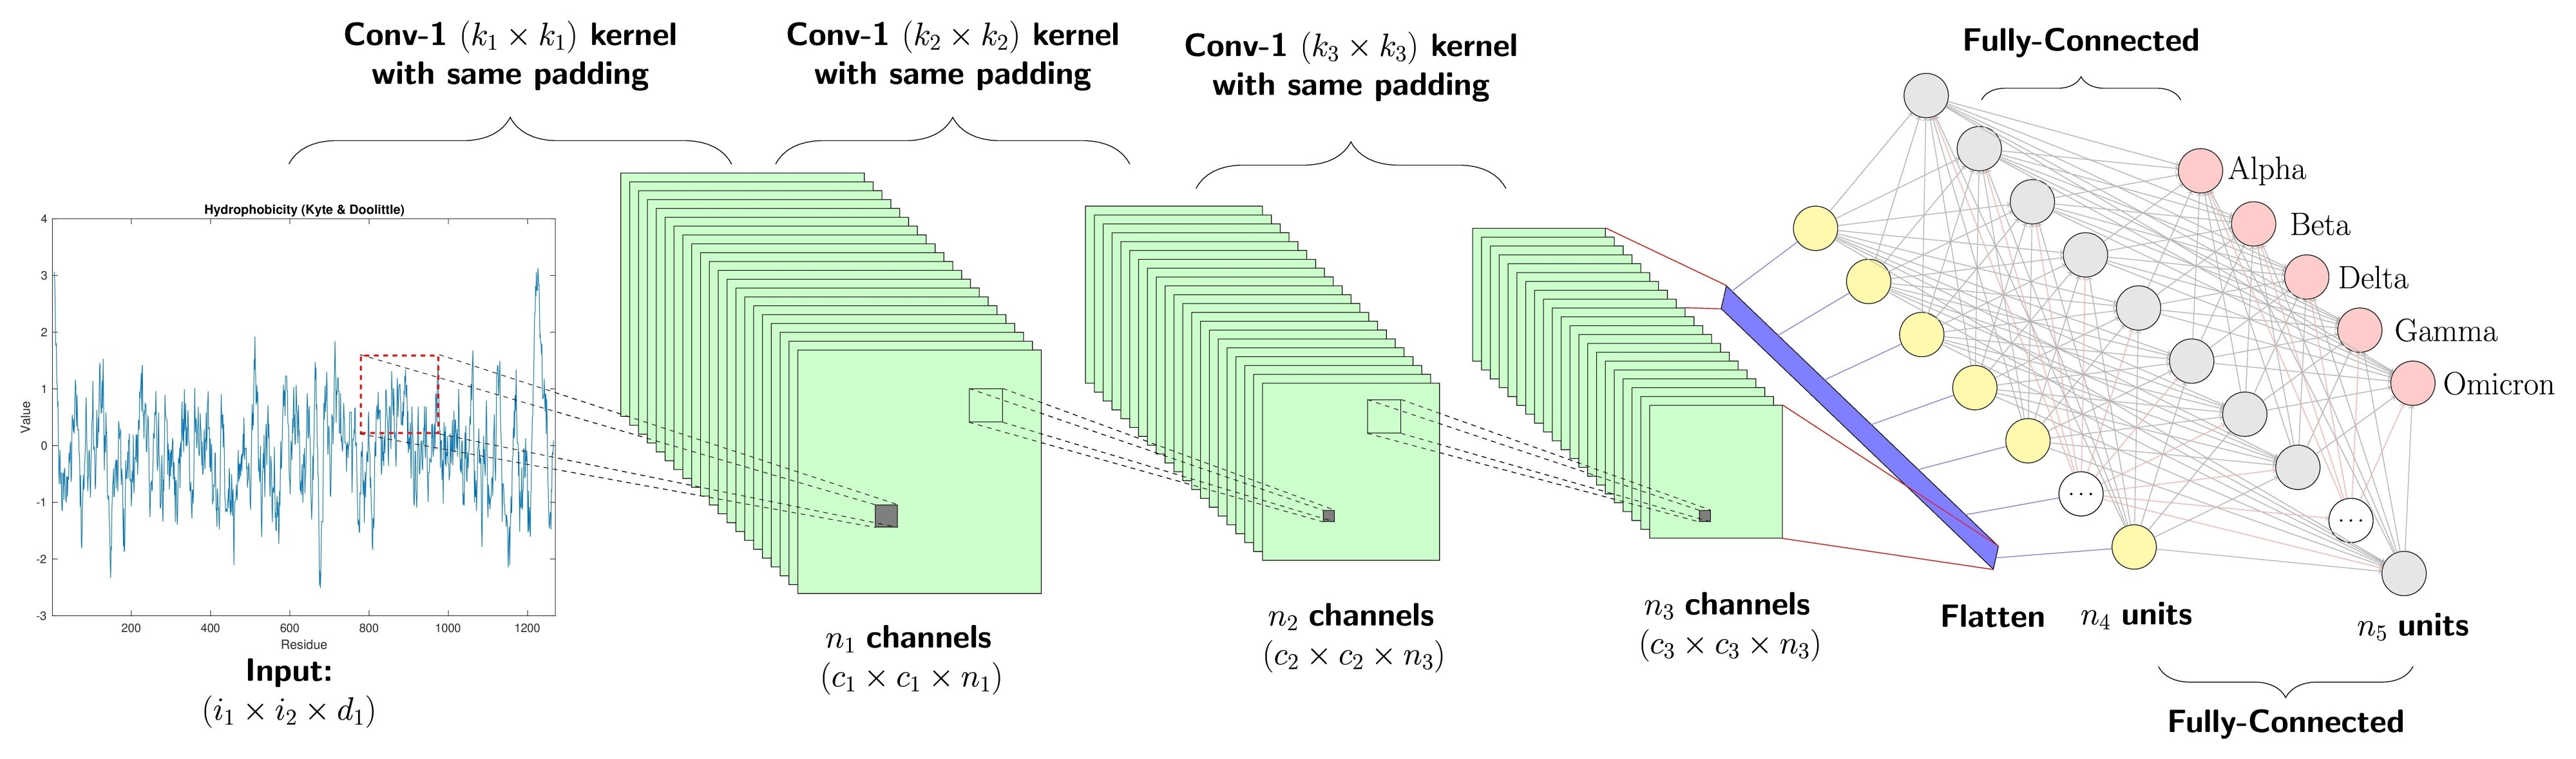
\includegraphics[width=\textwidth]{images/2_2_convolution.jpeg}
\caption{Phép tích chập và gộp.}
\label{fig:cnn_ops}
\end{figure}
\end{column}
\end{columns}
\end{frame}

\begin{frame}
\frametitle{Mô hình Học sâu: Vision Transformer}
\begin{columns}
\begin{column}{0.5\textwidth}
\begin{itemize}
\item \textbf{Vision Transformer (ViT)}: Chia ảnh thành \textbf{miếng vá}, xử lý như token.
\item \textbf{Tự chú ý (Self-Attention)}:
\begin{equation}
\footnotesize
\text{Attention}(Q, K, V) = \text{softmax}\left(\frac{QK^T}{\sqrt{d_k}}\right)V
\end{equation}
\item Học quan hệ toàn cục, vượt giới hạn của CNN.
\end{itemize}
\end{column}

\begin{column}{0.45\textwidth}
\begin{figure}
\centering
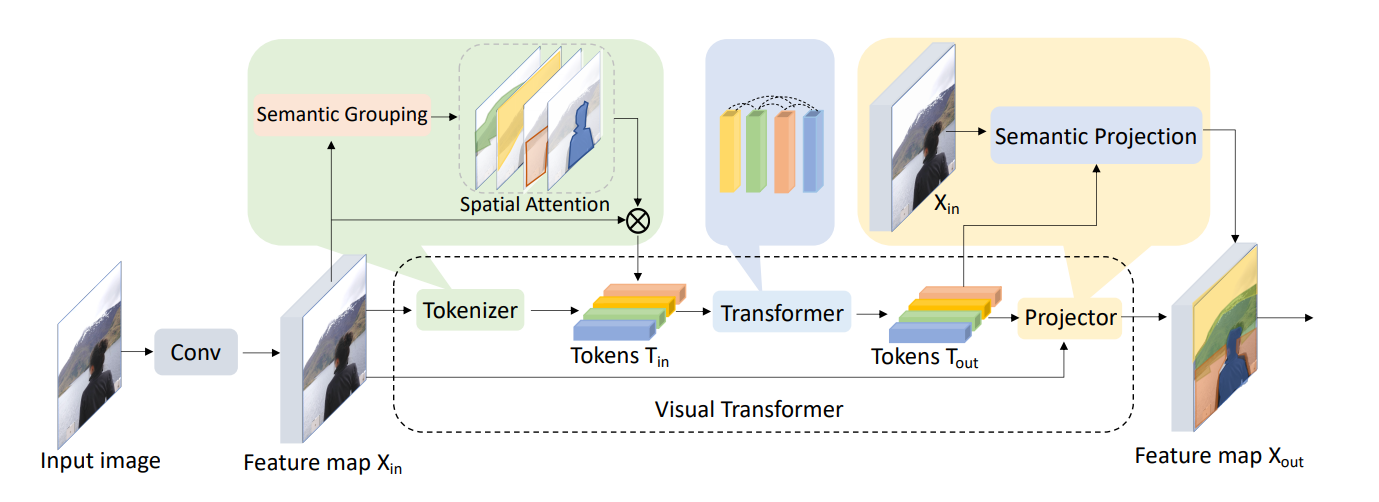
\includegraphics[width=\textwidth]{images/visual_transformer.png}
\caption{Kiến trúc ViT.}
\label{fig:vit_arch}
\end{figure}
\end{column}
\end{columns}
\end{frame}

\begin{frame}
\frametitle{Tập dữ liệu và Metrics Đánh giá}
\begin{block}{Tập dữ liệu}
\begin{itemize}
\item \textbf{ImageNet}: Phân loại ảnh (>14 triệu ảnh).
\item \textbf{COCO}: Phát hiện, phân đoạn đối tượng.
\item \textbf{MPII, COCO Keypoints}: Ước lượng tư thế người (HPE).
\end{itemize}
\end{block}

\begin{block}{Metrics đánh giá}
\begin{itemize}
\item \textbf{IoU}: Đo độ trùng khớp hộp giới hạn.
\item \textbf{mAP}: Trung bình độ chính xác cho phát hiện đối tượng.
\item \textbf{F1-score}: Cân bằng Precision và Recall.
\item \textbf{OKS}: Đo độ chính xác khớp trong HPE.
\end{itemize}
\end{block}
\end{frame}

\subsection{Nhận diện tư thế người}
% Slide 1: Section Overview
\begin{frame}{Nhận diện Tư thế Người và Phát hiện Té ngã}
    \begin{block}{Tổng quan}
        Hệ thống tích hợp nhận diện tư thế (MediaPipe Pose) và phát hiện té ngã dựa trên đặc trưng động học/tư thế.
        \begin{itemize}
            \item Ứng dụng: Giám sát an toàn, phát hiện té ngã.
            \item Nền tảng: Thị giác máy tính thời gian thực.
        \end{itemize}
    \end{block}
\end{frame}

% Slide 2: Nhận diện Tư thế Người
\begin{frame}{Nhận diện Tư thế Người}
\begin{columns}[T]
    \begin{column}{0.45\textwidth}
        \centering
        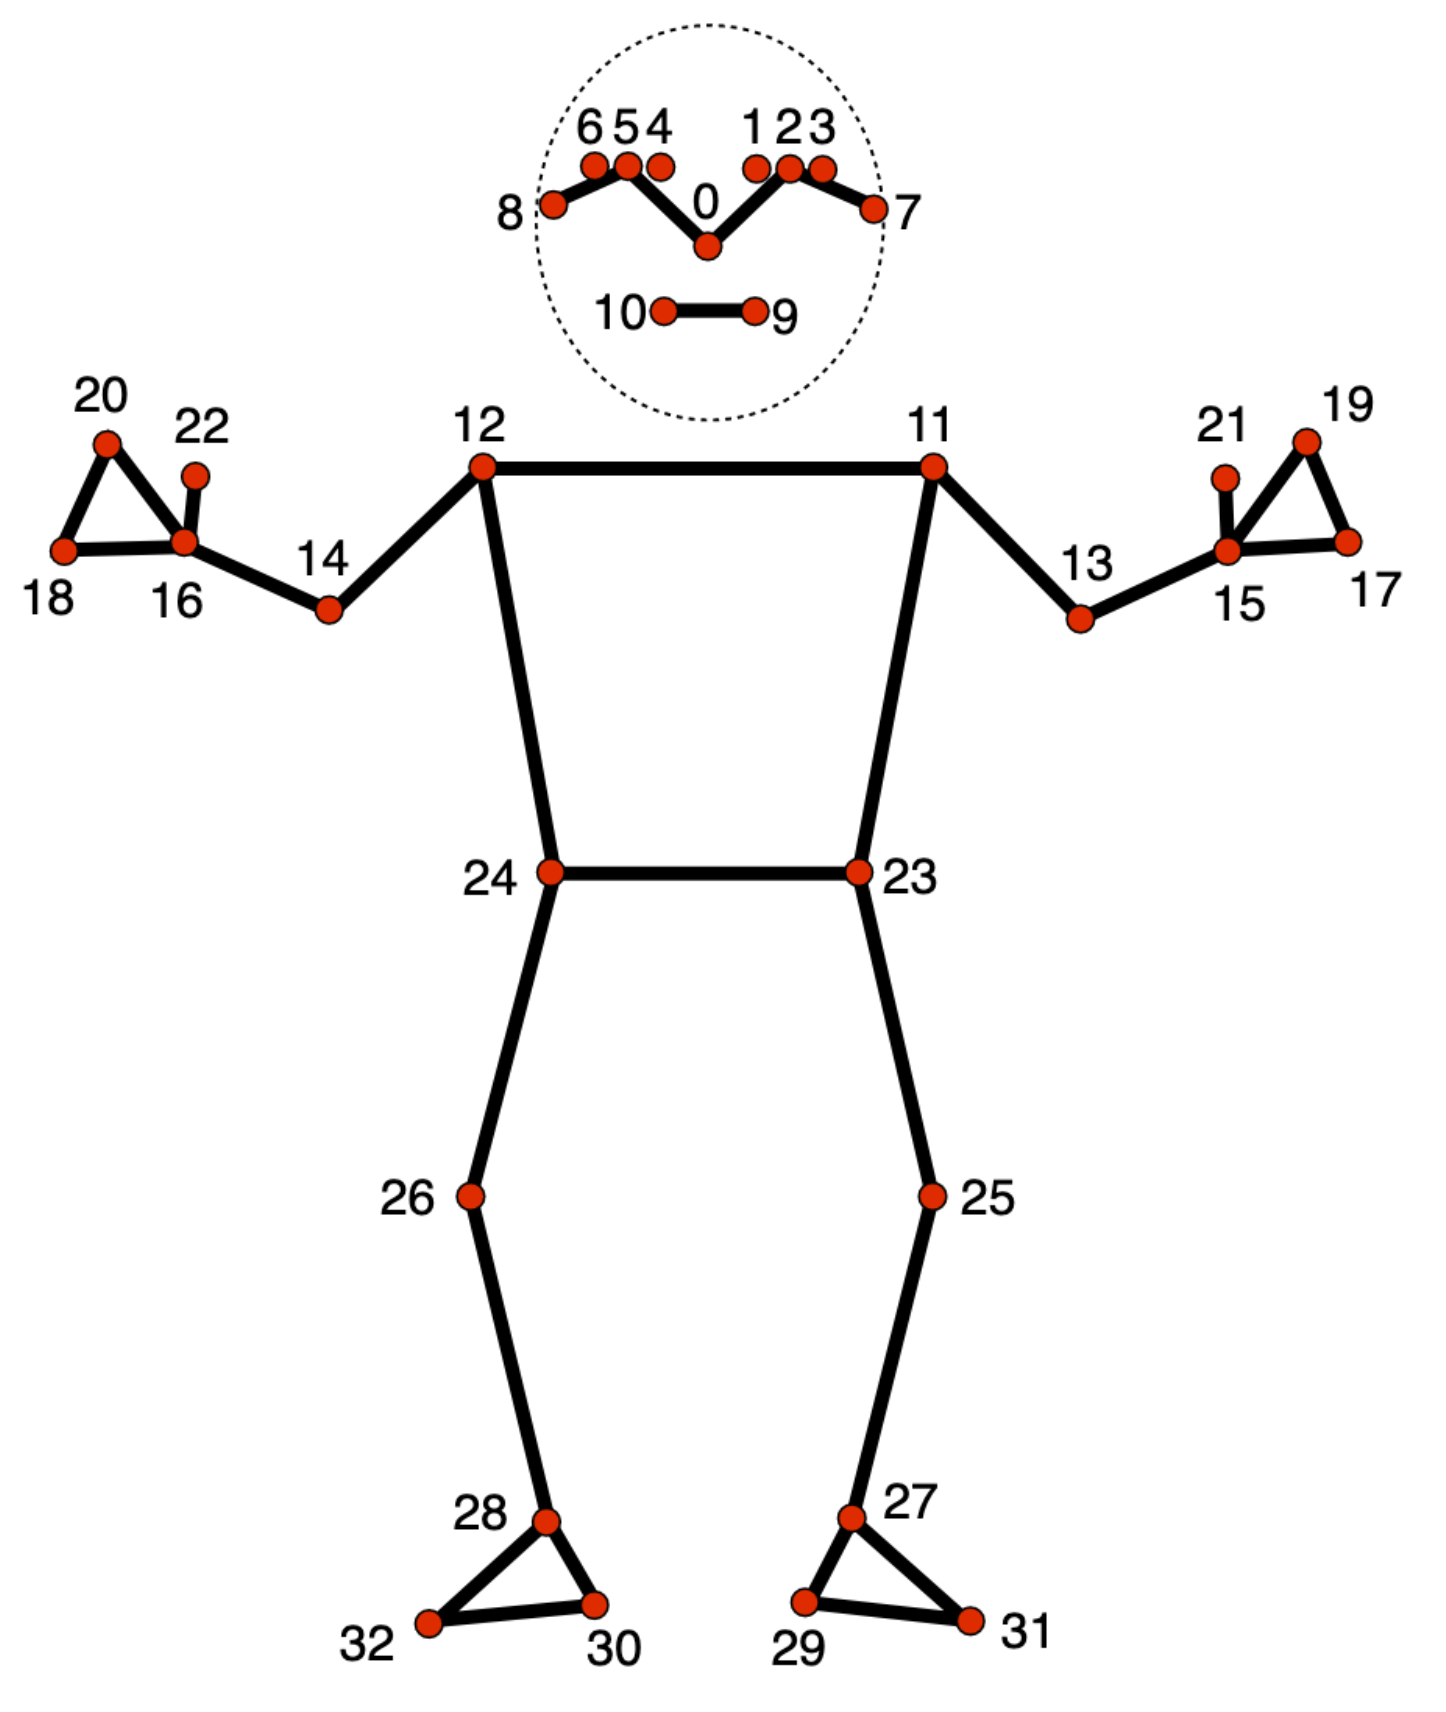
\includegraphics[height=0.8\textheight, keepaspectratio]{pose_landmarks_index.png}
        \vspace{0.2cm}
        {\small Keypoints cơ bản trong HPE (Human Pose Estimation).}
    \end{column}

    \begin{column}{0.55\textwidth}
        \begin{block}{Khái niệm}
            Ước lượng vị trí khớp từ hình ảnh/video:
            \[
                \mathcal{K} = \{k_i = (x_i, y_i, z_i, c_i)\}
            \]
            \small{\textit{($c_i$ là confidence score cho mỗi keypoint).}}
        \end{block}

        \begin{alertblock}{Phương pháp}
            \begin{itemize}
                \item \textbf{Top-down:} Phát hiện người trước, sau đó keypoints (MediaPipe).
                \item \textbf{Bottom-up:} Keypoints trước, nhóm thành người sau (OpenPose).
            \end{itemize}
        \end{alertblock}
    \end{column}
\end{columns}
\end{frame}

% Slide 3: MediaPipe Pose – Kiến trúc BlazePose
\begin{frame}{MediaPipe Pose – Kiến trúc BlazePose}
    \begin{block}{Kiến trúc BlazePose}
        BlazePose tối ưu HPE 3D với:
        \begin{itemize}
            \item \textbf{Nodes:} Các module xử lý tín hiệu hình ảnh.
            \item \textbf{Edges:} Luồng dữ liệu đồng bộ giữa các module.
        \end{itemize}
        \small{\textit{(Nodes = các bước tính toán; Edges = kết nối dữ liệu giữa các bước).}}
    \end{block}
\end{frame}

% Slide 4: MediaPipe Pose – Thành phần & Hậu xử lý
\begin{frame}{MediaPipe Pose – Thành phần & Hậu xử lý}
    \begin{exampleblock}{Thành phần chính}
        \begin{itemize}
            \item \textbf{Detection:} ROI từ ảnh RGB, phát hiện người.
            \item \textbf{Landmark:} 33 keypoints 3D, Loss: $\mathcal{L} = \sum \lambda_i \mathcal{L}_i$.
            \item \textbf{Tracking:} Dự đoán vị trí ROI cho khung tiếp theo.
        \end{itemize}
        \small{\textit{(Landmark 3D giúp đánh giá tư thế và động tác).}}
    \end{exampleblock}

    \begin{alertblock}{Hậu xử lý}
        \begin{itemize}
            \item \textbf{One Euro Filter:} Làm mịn nhiễu trong dữ liệu keypoints.
            \item \textbf{Chuẩn hóa $z$:} Dựa trên hông, tăng độ chính xác 3D.
        \end{itemize}
    \end{alertblock}
\end{frame}


% Slide 5: Thuật toán Phát hiện Té ngã
\begin{frame}{Thuật toán Phát hiện Té ngã}
    \begin{columns}[T]
        \column{0.5\textwidth}
        \begin{block}{Đặc trưng Động học}
            \begin{itemize}
                \item \textbf{Vận tốc COM:} $\vec{v}_{\text{COM}} = \frac{\Delta \vec{p}}{\Delta t}$
                \item \textbf{Gia tốc:} $a = \frac{\|\Delta \vec{v}\|}{\Delta t}$
            \end{itemize}
        \end{block}
        \begin{block}{Đặc trưng Tư thế}
            \begin{itemize}
                \item \textbf{AR (Aspect Ratio):} Tăng khi người nằm ngang
                \item \textbf{$\theta_{\text{body}}$:} Góc vai-hông
                \item \textbf{$\Delta h_{\text{head}}$:} Giảm chiều cao đầu
            \end{itemize}
            \small{\textit{(AR, $\theta$, $\Delta h$ giúp xác định tư thế bất thường).}}
        \end{block}

        \column{0.5\textwidth}
        \begin{alertblock}{Ba Giai đoạn Phát hiện}
            \begin{enumerate}
                \item \textbf{Sớm:} Tốc độ/gia tốc COM cao
                \item \textbf{Xác nhận:} AR, $\theta_{\text{body}}$ chỉ nằm ngang
                \item \textbf{Bất động:} Chuyển động $< M_{th}$
            \end{enumerate}
        \end{alertblock}
    \end{columns}
\end{frame}



\subsection{Cơ sở lý thuyết xây dựng phần cứng}

% Slide 1: Tổng quan hệ thống
\begin{frame}{Tổng quan Kiến trúc Hệ thống Phát hiện Té ngã}
\begin{block}{Phân loại hệ thống}
\begin{itemize}
\item \textbf{Dựa trên Camera}: Xử lý hình ảnh cố định, yêu cầu máy chủ mạnh
\item \textbf{Dựa trên Thiết bị đeo}: Cảm biến IMU, ESP32, truyền thông di động
\end{itemize}
\end{block}

\begin{block}{Ba thành phần cốt lõi}
\begin{enumerate}
\item \textbf{Thiết bị Thu thập Dữ liệu}: IMU, Camera, GPS
\item \textbf{Máy chủ/Xử lý}: Phân tích dữ liệu, Học sâu
\item \textbf{Truyền thông}: Wi-Fi, 4G/LTE đảm bảo kết nối
\end{enumerate}
\end{block}
\end{frame}

% Slide 8: Môi trường phát triển

\begin{frame}{Môi trường Phát triển (ESP-IDF)}
\begin{columns}
\column{0.5\textwidth}
\begin{block}{Đặc trưng của ESP-IDF}
\begin{itemize}
    \item \textbf{Build system CMake + Kconfig} 
          – cấu hình linh hoạt, dễ mở rộng component
    \item \textbf{FreeRTOS tích hợp sẵn} 
          – quản lý đa nhiệm trên 2 lõi Xtensa
    \item \textbf{Driver cấp thấp} 
          – I2C, SPI, UART, PWM, GPIO được tối ưu cho ESP32
    \item \textbf{Hỗ trợ mạng phong phú} 
          – Wi-Fi, Bluetooth, TCP/IP stack, MQTT, HTTP(S)
\end{itemize}
\end{block}

\column{0.5\textwidth}
\begin{exampleblock}{Lợi ích cho hệ thống Phát hiện Té ngã}
\begin{itemize}
    \item Quản lý \textbf{đa component} (IMU, SIM4G, LED, Fall Logic) độc lập
    \item Thực thi \textbf{song song}: 
          lõi 1 xử lý cảm biến, lõi 2 lo truyền thông
    \item Hỗ trợ \textbf{OTA update} để nâng cấp firmware từ xa
    \item Debug chuyên nghiệp: \texttt{idf.py monitor}, gdbstub, logging
\end{itemize}
\end{exampleblock}
\end{columns}
\end{frame}
% Slide 2: ESP32
\begin{frame}{Vi điều khiển ESP32}
\begin{columns}
\column{0.6\textwidth}
\begin{block}{Đặc điểm chính}
\begin{itemize}
\item Lõi kép Xtensa LX6, FreeRTOS
\item Wi-Fi + Bluetooth tích hợp
\item Hỗ trợ MQTT, HTTP
\end{itemize}
\end{block}

\begin{block}{Phân công nhiệm vụ}
\begin{itemize}
\item \textbf{Lõi 1}: Xử lý thời gian thực (IMU, Kalman Filter)
\item \textbf{Lõi 2}: Truyền thông không dây
\end{itemize}
\end{block}

\column{0.4\textwidth}
\begin{center}
    % Hiển thị hình ESP32 thay cho TikZ
    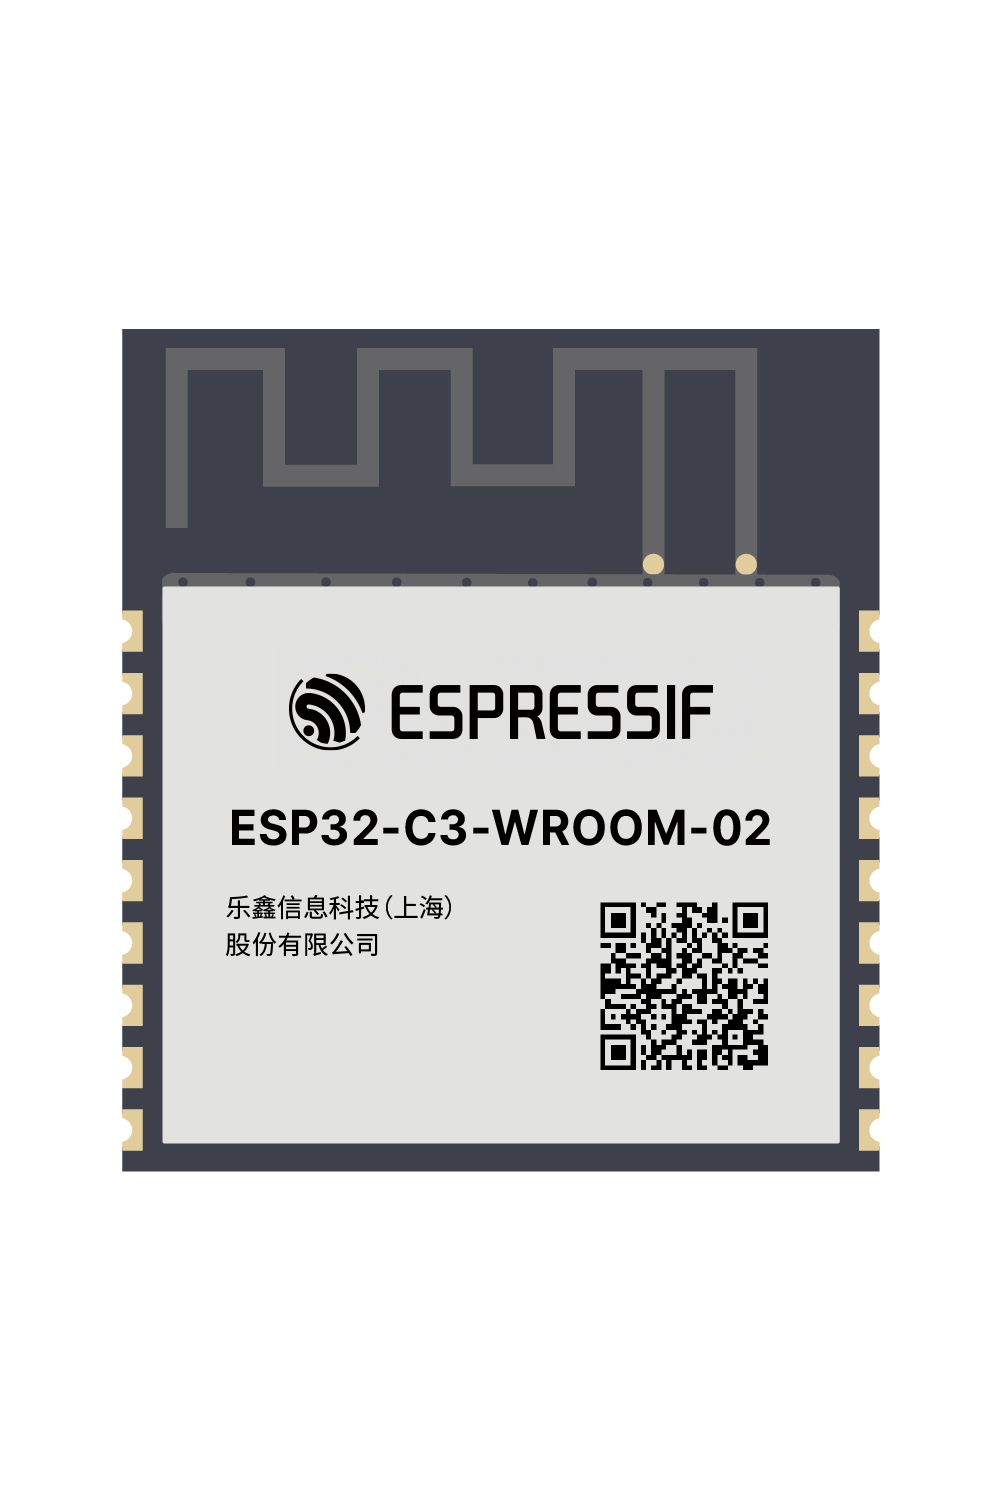
\includegraphics[width=\linewidth]{images/esp32_c3.png}
\end{center}
\end{columns}
\end{frame}

% Slide 3: IMU & GPS
\begin{frame}{Cảm biến IMU và GPS}
\begin{columns}
\column{0.5\textwidth}
\begin{block}{IMU}
\begin{itemize}
\item Gia tốc kế $\mathbf{a}=[a_x,a_y,a_z]$
\item Con quay hồi chuyển $\boldsymbol{\omega}=[\omega_x,\omega_y,\omega_z]$
\item Từ kế – xác định hướng
\item Fusion: Kalman/Madgwick
\end{itemize}
\end{block}

\column{0.5\textwidth}
\begin{exampleblock}{GPS}
\begin{itemize}
\item Module NEO-6M / EC800K
\item Định vị NMEA, tọa độ cứu hộ
\item Kết hợp truyền thông SMS/4G
\end{itemize}
\end{exampleblock}
\end{columns}
\end{frame}


% Slide 5: Edge vs Cloud
\begin{frame}{Xử lý tại Biên và Máy chủ }
\begin{columns}
\column{0.5\textwidth}
\begin{block}{Edge (ESP32)}
\begin{itemize}
\item Xử lý IMU thời gian thực
\item Phát hiện té ngã sơ cấp
\item Truyền dữ liệu JSON/MQTT
\end{itemize}
\end{block}

\column{0.5\textwidth}
\begin{block}{Cloud/Server}
\begin{itemize}
\item Xử lý ảnh từ Camera (ESP32-S3 + OV5640)
\item TensorFlow/PyTorch, OpenCV
\end{itemize}
\end{block}
\end{columns}
\end{frame}
%---------

\begin{frame}{Hệ thống Truyền thông và Logic Hoạt động}
%---------------- Cột Wi-Fi/4G ----------------%
\begin{columns}[T]
    \column{0.5\textwidth}
    \begin{alertblock}{Wi-Fi (chính)}
        \begin{itemize}
            \item Truyền tải dung lượng lớn (ảnh/video)
            \item MQTT với máy chủ
            \item Độ trễ thấp
        \end{itemize}
    \end{alertblock}

    \column{0.5\textwidth}
    \begin{alertblock}{4G/LTE (dự phòng)}
        \begin{itemize}
            \item SMS/cuộc gọi khẩn
            \item Định vị GPS
            \item Hoạt động khi Wi-Fi lỗi
        \end{itemize}
    \end{alertblock}
\end{columns}

\vspace{0.3cm}

%---------------- Logic hoạt động ----------------%
\textbf{Logic Hoạt động Hệ thống:}
\begin{enumerate}
    \item ESP32 thu thập dữ liệu IMU/Camera
    \item Phát hiện té ngã sơ cấp tại biên
    \item Truyền dữ liệu lên máy chủ (ưu tiên Wi-Fi, dự phòng 4G)
    \item Máy chủ xử lý tin và phát cảnh báo
    \item Kích hoạt cảnh báo (SMS/cuộc gọi)
\end{enumerate}
\end{frame}

\begin{frame}{06_background_summary}
  % TODO: Add content for 06_background_summary
\end{frame}


% --- Methodology ---
\section{III-THIẾT KẾ VÀ TRIỂN KHAI}
% Slide 1: Kiến trúc tổng quan
\subsection{Tổng quan kiến trúc}
\begin{frame}
\frametitle{Kiến trúc Hệ thống FDAS}

\begin{figure}[h]
\centering
\includegraphics[width=0.85\textwidth]{images/3_1_system_architecture_diagram.pdf}
\caption{Sơ đồ Kiến trúc Hệ thống Phát hiện té ngã và Cảnh báo}
\end{figure}

\begin{block}{4 lớp chính}
\begin{itemize}
\item \textbf{Lớp Thiết bị/Biên}: Thu thập dữ liệu
\item \textbf{Lớp Kết nối}: Truyền tải dữ liệu  
\item \textbf{Lớp Xử lý/Đám mây}: Xử lý và ra quyết định
\item \textbf{Lớp Ứng dụng/UI}: Giao diện người dùng
\end{itemize}
\end{block}

\end{frame}

% Slide 2: Lớp Thiết bị/Biên
\begin{frame}
\frametitle{Lớp Thiết bị/Biên}

\begin{columns}
\column{0.5\textwidth}
\begin{block}{ESP32 Module}
\begin{itemize}
\item Cảm biến gia tốc \& con quay
\item Phát hiện mẫu chuyển động té ngã
\end{itemize}
\end{block}

\begin{block}{Module GPS}
\begin{itemize}
\item Thu thập vị trí địa lý
\item Hỗ trợ giám sát ngoài trời
\end{itemize}
\end{block}

\column{0.5\textwidth}
\begin{block}{IP Camera}
\begin{itemize}
\item Luồng video liên tục
\item Giám sát trong nhà
\end{itemize}
\end{block}

\vspace{1cm}
\begin{alertblock}{Đặc điểm}
2 nguồn dữ liệu độc lập
\end{alertblock}

\end{columns}

\end{frame}

% Slide 3: Lớp Kết nối
\begin{frame}
\frametitle{Lớp Kết nối}

\begin{columns}
\column{0.5\textwidth}
\begin{block}{Kênh truyền}
\begin{itemize}
\item Wi-Fi/4G/LTE
\item Đảm bảo kết nối liên tục
\end{itemize}
\end{block}

\column{0.5\textwidth}
\begin{block}{MQTT Broker}
\begin{itemize}
\item Mô hình Publish/Subscribe
\item ESP32 → JSON data
\item Server nhận real-time
\end{itemize}
\end{block}
\end{columns}

\end{frame}

% Slide 4: Lớp Xử lý/Đám mây
\begin{frame}
\frametitle{Lớp Xử lý/Đám mây}

\begin{block}{Main Processing Server (Python)}
\begin{itemize}
\item \textbf{MQTT Client}: Subscribe dữ liệu từ ESP32
\item \textbf{AI \& Image Processing}: YOLO model xử lý video
\item \textbf{Business Logic}: Kết hợp 2 luồng dữ liệu → Quyết định cảnh báo
\end{itemize}
\end{block}

\begin{columns}
\column{0.5\textwidth}
\begin{block}{Asterisk Server}
\begin{itemize}
\item Tổng đài PBX
\item Cuộc gọi khẩn cấp (SIP)
\end{itemize}
\end{block}

\column{0.5\textwidth}
\begin{block}{Telegram Bot API}
\begin{itemize}
\item Tin nhắn/hình ảnh
\item Thông báo nhóm
\end{itemize}
\end{block}
\end{columns}

\end{frame}

% Slide 5: Lớp Ứng dụng/UI
\begin{frame}
\frametitle{Lớp Ứng dụng/Giao diện}

\begin{columns}
\column{0.33\textwidth}
\begin{block}{Mobile/Web App}
\begin{itemize}
\item Dashboard
\item Lịch sử sự kiện
\item Cấu hình
\end{itemize}
\end{block}

\column{0.33\textwidth}
\begin{block}{SIP Client}
\begin{itemize}
\item Linphone/Zoiper
\item Nhận cuộc gọi báo động
\end{itemize}
\end{block}

\column{0.33\textwidth}
\begin{block}{Telegram}
\begin{itemize}
\item Thông báo trực tiếp
\item Tương tác 2 chiều
\end{itemize}
\end{block}
\end{columns}

\vspace{0.5cm}
\begin{center}
\textbf{Cảnh báo đa kênh}: Gọi thoại + Nhắn tin
\end{center}

\end{frame}


\subsection{THỰC HIỆN PHẦN CỨNG}
% Slide 1: Tổng quan phần cứng
\begin{frame}
\frametitle{Thực hiện Phần cứng FDAS}

\begin{block}{Kiến trúc mô-đun}
Hệ thống gồm 2 module hoạt động độc lập:
\begin{itemize}
\item \textbf{Module I}: Thiết bị đeo/Cảm biến - Thu thập chuyển động \& định vị
\item \textbf{Module II}: Camera giám sát - Xác nhận sự kiện qua hình ảnh
\end{itemize}
\end{block}

\begin{columns}
\column{0.5\textwidth}
\begin{alertblock}{Ưu điểm}
\begin{itemize}
\item Linh hoạt triển khai
\item Giám sát phạm vi rộng  
\item Duy trì hoạt động khi 1 module lỗi
\end{itemize}
\end{alertblock}

\column{0.5\textwidth}
\begin{block}{Nguyên lý}
2 nguồn dữ liệu độc lập tăng độ tin cậy phát hiện
\end{block}
\end{columns}

\end{frame}

% Slide 2: Module I - Sơ đồ và sản phẩm thực tế
\begin{frame}
\frametitle{Module I: Thiết bị đeo/Cảm biến}

\begin{columns}
\column{0.5\textwidth}
\begin{figure}[h]
\centering
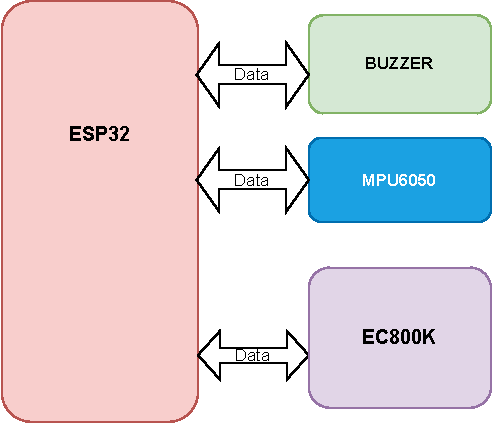
\includegraphics[width=\textwidth]{images/module1_block_diagram-crop.pdf}
\caption{Sơ đồ khối Module I}
\end{figure}

\column{0.5\textwidth}
\begin{figure}[h]
\centering
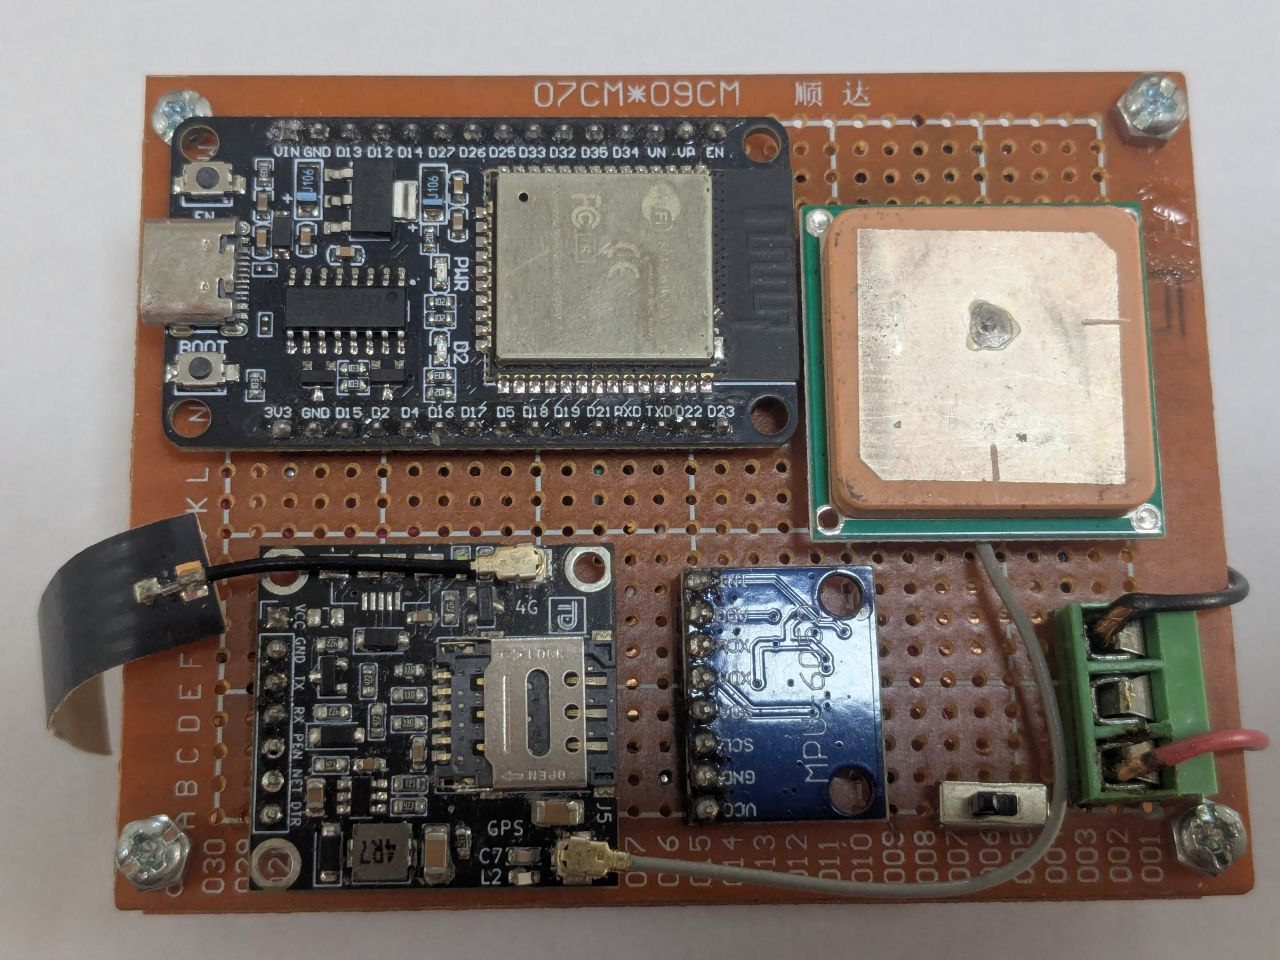
\includegraphics[width=\textwidth]{images/real_board1.jpg}
\caption{Module I thực tế}
\end{figure}
\end{columns}

\begin{block}{Thành phần chính}
\textbf{ESP32-DevKitC-1} (Wi-Fi/BLE) • \textbf{MPU6050} (IMU 6 trục) • \textbf{GPS/4G EC800K} (Định vị) • \textbf{Buzzer/LED} (Cảnh báo)
\end{block}

\end{frame}

% Slide 3: Module II - Camera
\begin{frame}
\frametitle{Module II: Camera giám sát}

\begin{columns}
\column{0.6\textwidth}
\begin{block}{Thành phần chính}
\begin{itemize}
\item \textbf{ESP32-S3-N16R8}:
  \begin{itemize}
  \item Vi điều khiển mạnh mẽ
  \item Tích hợp PSRAM
  \item Giao diện camera chuyên dụng
  \end{itemize}
\item \textbf{Camera OV5640}:
  \begin{itemize}
  \item Cảm biến 5MP
  \item Đa kích thước (QQVGA-UXGA)
  \item Bus 8-bit, 20MHz
  \end{itemize}
\end{itemize}
\end{block}

\column{0.4\textwidth}
\begin{figure}[h]
\centering
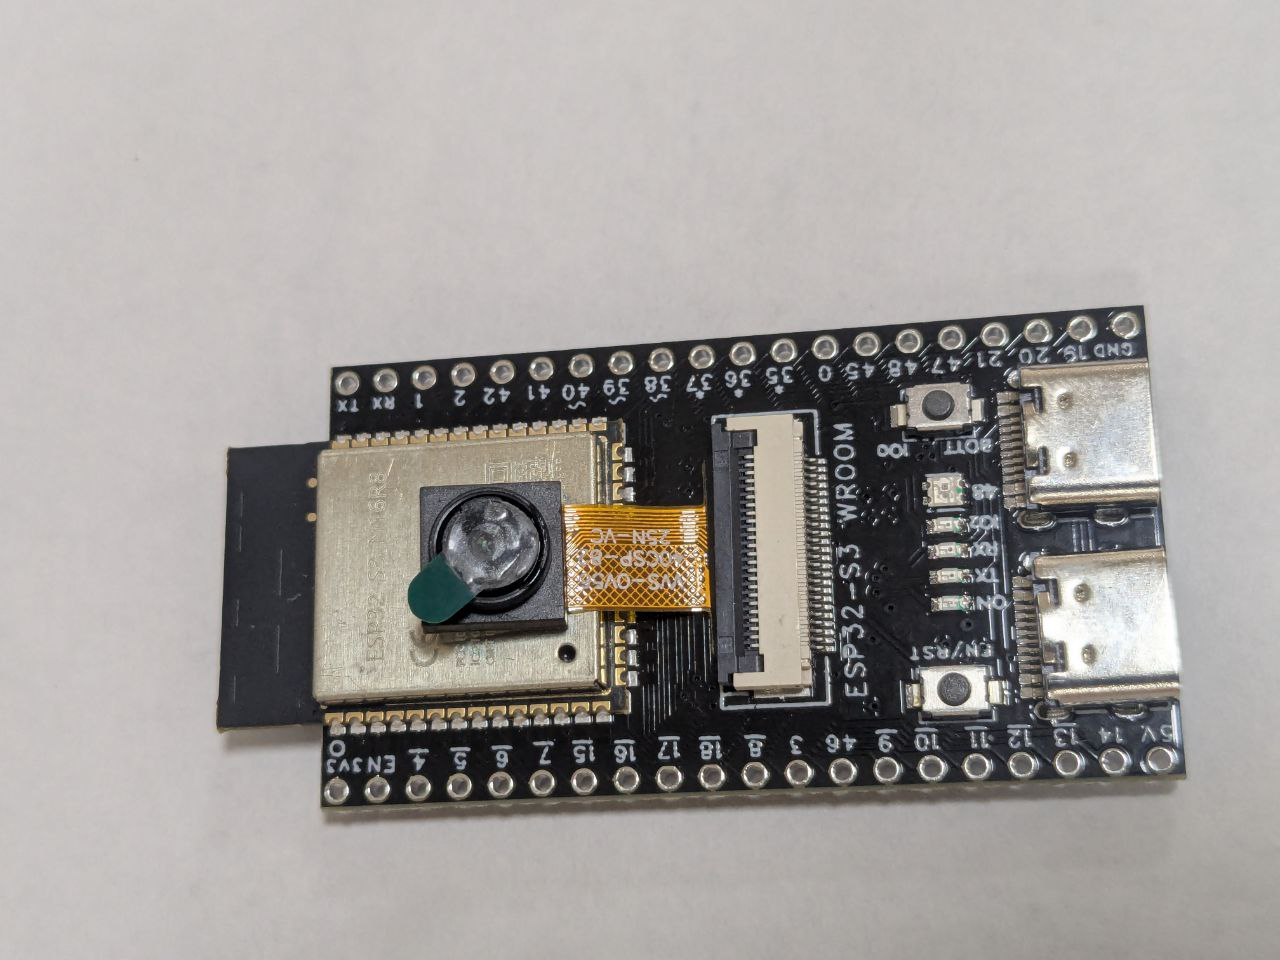
\includegraphics[width=\textwidth]{images/real_board2.jpg}
\caption{Module II thực tế}
\end{figure}
\end{columns}

\end{frame}

% Slide 4: Kết nối phần cứng Module II
\begin{frame}
\frametitle{Kết nối ESP32-S3 ↔ OV5640}

\begin{table}[h]
\centering
\caption{Sơ đồ kết nối chân}
\begin{tabular}{|l|c|l|}
\hline
\textbf{Chức năng} & \textbf{Chân ESP32-S3} & \textbf{Mô tả} \\
\hline
XCLK & 15 & Xung nhịp camera \\
SIOD (SDA) & 4 & Dữ liệu I2C \\
SIOC (SCL) & 5 & Xung nhịp I2C \\
D0-D7 & 11,9,8,10,12,18,17,16 & Bus dữ liệu 8-bit \\
VSYNC & 6 & Đồng bộ dọc \\
HREF & 7 & Tham chiếu ngang \\
PCLK & 13 & Xung nhịp điểm ảnh \\
\hline
\end{tabular}
\end{table}

\begin{alertblock}{Giao tiếp}
SCCB (tương tự I2C) cho cấu hình + Bus song song 8-bit cho dữ liệu
\end{alertblock}

\end{frame}

% Slide 6: Tổng hợp phần cứng - Phần 1
\begin{frame}
\frametitle{Chi phí Phần cứng - Module I}

\begin{table}[h]
\centering
\small
\begin{tabular}{|l|l|r|}
\hline
\textbf{Linh kiện} & \textbf{Chức năng} & \textbf{Giá (VNĐ)} \\
\hline
ESP32-DevKitC-1 & Vi điều khiển chính & 110.000 - 125.000 \\
MPU6050 & Cảm biến IMU 6 trục & 45.000 - 55.000 \\
GPS antenna & Anten nhận GPS & 35.000 - 60.000 \\
GPS/4G EC800K & Định vị \& gửi cảnh báo & ~240.000 \\
Buzzer & Cảnh báo âm thanh & 5.000 - 10.000 \\
\hline
\textbf{Tổng Module I} & & \textbf{~435.000 - 490.000} \\
\hline
\end{tabular}
\end{table}

\begin{block}{Đặc điểm Module I}
Thiết bị đeo nhỏ gọn, chi phí hợp lý, tích hợp đầy đủ cảm biến
\end{block}

\end{frame}

% Slide 7: Tổng hợp phần cứng - Phần 2  
\begin{frame}
\frametitle{Chi phí Phần cứng - Module II}

\begin{table}[h]
\centering
\begin{tabular}{|l|l|r|}
\hline
\textbf{Linh kiện} & \textbf{Chức năng} & \textbf{Giá (VNĐ)} \\
\hline
ESP32-S3-N16R8 & Vi điều khiển xử lý ảnh & 275.000 - 300.000 \\
Camera OV5640 & Cảm biến hình ảnh 5MP & 150.000 - 200.000 \\
\hline
\textbf{Tổng Module II} & & \textbf{~425.000 - 500.000} \\
\hline
\hline
\textbf{TỔNG HỆ THỐNG} & & \textbf{~860.000 - 990.000} \\
\hline
\end{tabular}
\end{table}

\begin{columns}
\column{0.5\textwidth}
\begin{block}{Module II}
Camera giám sát cố định, xử lý hình ảnh AI
\end{block}

\column{0.5\textwidth}
\begin{alertblock}{Tổng kết}
Hệ thống hoàn chỉnh < 1 triệu VNĐ
\end{alertblock}
\end{columns}

\end{frame}

\subsection{Triển khai phần mềm}
\begin{frame}
\frametitle{Tổng quan Triển khai Phần mềm toàn bộ Hệ thống}

\begin{table}[htbp]
\centering
\small
\begin{tabular}{|l|l|l|l|}
\hline
\textbf{Thành phần} & \textbf{Nền tảng} & \textbf{Công nghệ chính} & \textbf{Chức năng} \\
\hline
\textbf{Module I} & ESP32 & ESP-IDF, C/C++ & Cảm biến đeo, phát hiện ngã \\
\hline
\textbf{Module II} & ESP32 & ESP-IDF, OpenCV & Camera giám sát \\
\hline
\textbf{Server} & Linux & Python, MQTT & Xử lý trung tâm, AI \\
\hline
\textbf{Asterisk} & Linux Mint 21 & PJSIP, AMI & Hệ thống VoIP \\
\hline
\end{tabular}
\end{table}

\vspace{0.3cm}

\begin{columns}[t]
\begin{column}{0.48\textwidth}
\begin{block}{Kiến trúc Phân tán}
\begin{itemize}
\item 4 thành phần độc lập
\item Giao tiếp qua giao thức chuẩn
\item Xử lý song song thời gian thực
\end{itemize}
\end{block}
\end{column}

\begin{column}{0.48\textwidth}
\begin{alertblock}{Nguyên tắc Thiết kế}
\begin{itemize}
\item Kiến trúc mô-đun
\item Khả năng mở rộng cao
\item Dễ bảo trì và nâng cấp
\end{itemize}
\end{alertblock}
\end{column}
\end{columns}

\vspace{0.3cm}
\begin{center}
\textit{\small Hệ thống tích hợp với khả năng cảnh báo đa dạng và xử lý thông minh}
\end{center}

\end{frame}

\begin{frame}{04_module_ast}
  % TODO: Add content for 04_module_ast
\end{frame}

% Slide: Luồng làm việc (OK - không cần sửa)
\begin{frame}[fragile]{Module cảm biến đeo: Luồng làm việc}
    \begin{block}{Quy trình}
        \begin{itemize}
            \item Điều phối từ thu thập dữ liệu cảm biến đến xử lý sự kiện và kích hoạt cảnh báo.
            \item Minh họa luồng làm việc:
        \end{itemize}
    \end{block}
    \begin{figure}
        \centering
        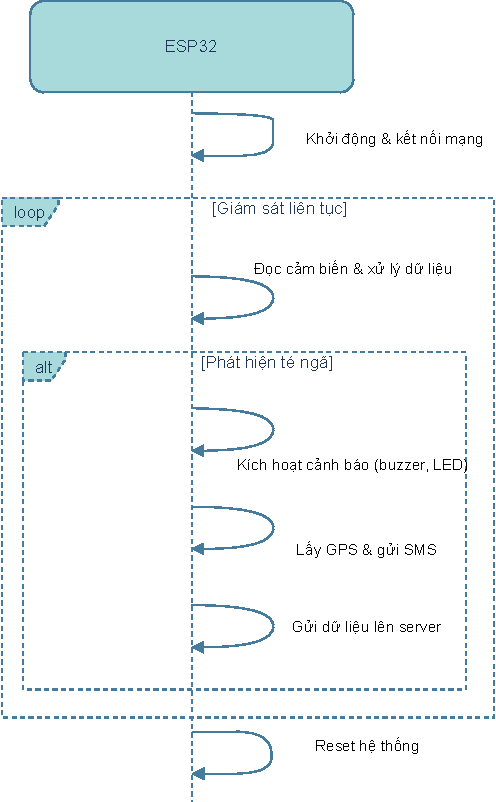
\includegraphics[width=0.9\textwidth,height=0.5\textheight,keepaspectratio]{images/module1_time_flow.pdf}
        \caption{Lưu đồ luồng làm việc của mô-đun phát hiện té ngã trên ESP32.}
        \label{fig:module1_flow}
    \end{figure}
\end{frame}

% Slide: Tổng quan mô-đun nhúng (OK - không cần sửa)
\begin{frame}{Module cảm biến đeo: Tổng quan mô-đun nhúng}
    \begin{block}{Tổng quan}
        \begin{itemize}
            \item Triển khai trên vi điều khiển \textbf{ESP32}: nút cảm biến và trung tâm cảnh báo.
            \item Chức năng chính:
            \begin{itemize}
                \item Thu thập dữ liệu chuyển động từ cảm biến.
                \item Phân tích thuật toán phát hiện té ngã.
                \item Cảnh báo thời gian thực: cục bộ (buzzer, LED) và từ xa (Wi-Fi/4G, MQTT, SMS).
            \end{itemize}
        \end{itemize}
    \end{block}
\end{frame}

% Slide: Môi trường phát triển (OK - không cần sửa)
\begin{frame}{Module cảm biến đeo: Môi trường phát triển}
    \begin{block}{Chi tiết}
        \begin{itemize}
            \item Phần mềm xây dựng trên \textbf{ESP-IDF} (Espressif IoT Development Framework).
            \item Hệ thống build: \textbf{CMake}, quản lý qua \texttt{idf\_component.yml}.
            \item API: UART, I2C, SPI, PWM, GPIO, Wi-Fi, MQTT, HTTP.
            \item Cấu hình qua \textbf{Kconfig}, lưu trong \texttt{sdkconfig}.
            \item Đảm bảo ổn định, mở rộng, tương thích driver.
        \end{itemize}
    \end{block}
\end{frame}

% Slide: Cấu trúc phần mềm
\begin{frame}[fragile]{Module cảm biến đeo: Cấu trúc project}
    \renewcommand{\baselinestretch}{0.8}
    \begin{minted}[fontsize=\scriptsize, breaklines, bgcolor=lightgray]{text}
mainproject/
├── main/
│   ├── main.c
│   ├── app_main.c
│   └── app_main.h
├── components/
│   ├── buzzer/
│   ├── comm/
│   ├── data_manager/
│   ├── event_handler/
│   ├── fall_logic/
│   ├── json_wrapper/
│   ├── led_indicator/
│   ├── mpu6050/
│   ├── sim4g_gps/
│   ├── user_mqtt/
│   └── wifi_connect/
    \end{minted}
    \renewcommand{\baselinestretch}{1.0}
\end{frame}

% Slide: Mô tả các thành phần (SỬA LẠI - tách thành 2 slide nếu cần)
\begin{frame}{Module cảm biến đeo: Mô tả các thành phần}
    \begin{columns}[t]
        \begin{column}{0.48\textwidth}
            \begin{block}{Thành phần chính}
                \begin{itemize}
                    \item \textbf{main.c}: Gọi \texttt{app\_main()}.
                    \item \textbf{app\_main.c/h}: Điều phối, khởi tạo.
                    \item \textbf{fall\_logic}: Thuật toán phát hiện té ngã.
                    \item \textbf{event\_handler}: Phản ứng sự kiện.
                    \item \textbf{mpu6050}: Driver cảm biến.
                \end{itemize}
            \end{block}
        \end{column}
        \begin{column}{0.48\textwidth}
            \begin{block}{Thành phần khác}
                \begin{itemize}
                    \item \textbf{buzzer, led\_indicator}: Cảnh báo cục bộ.
                    \item \textbf{sim4g\_gps, wifi\_connect}: Kết nối từ xa.
                    \item \textbf{user\_mqtt}: Giao tiếp MQTT.
                    \item \textbf{comm, data\_manager}: Quản lý giao tiếp.
                \end{itemize}
            \end{block}
        \end{column}
    \end{columns}
\end{frame}

% Slide: Sơ đồ khối phần mềm (OK - nhưng có thể điều chỉnh height nếu cần)
\begin{frame}[fragile]{Module cảm biến đeo: Sơ đồ khối phần mềm}
    \begin{figure}
        \centering
        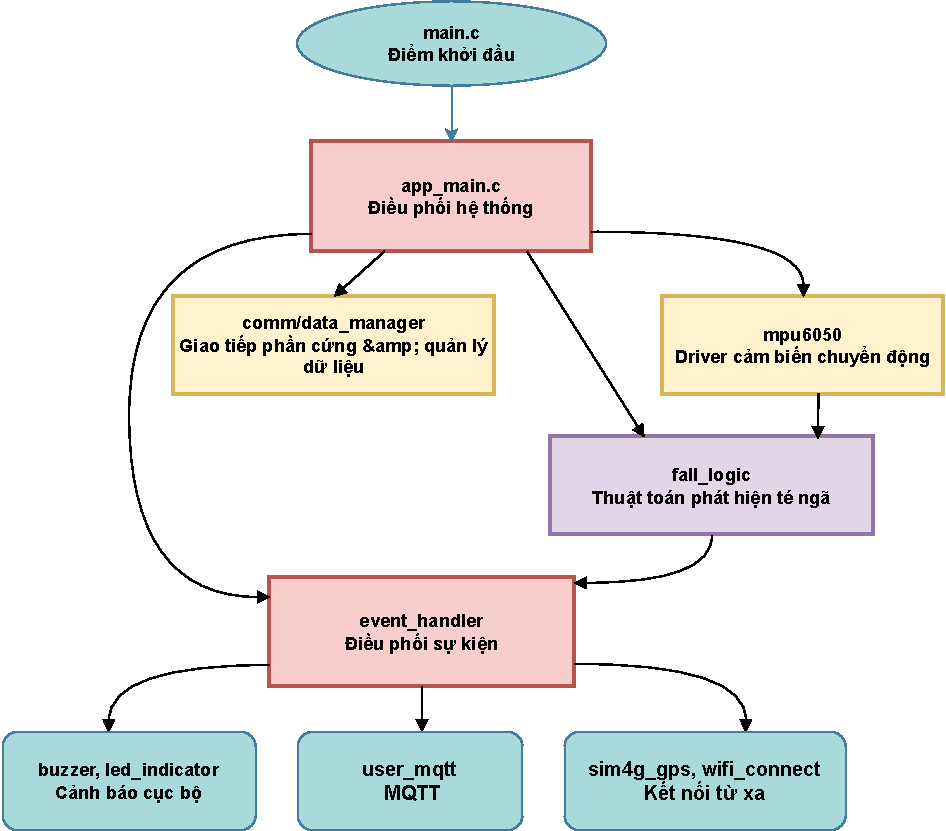
\includegraphics[width=0.85\textwidth,height=0.7\textheight,keepaspectratio]{images/module1_software_block-crop.pdf}
        \caption{Sơ đồ khối phần mềm của mô-đun nhúng ESP32.}
        \label{fig:module1_software_block}
    \end{figure}
\end{frame}

% Slide: Thuật toán phát hiện té ngã
\begin{frame}{Module cảm biến đeo: Thuật toán phát hiện té ngã}
    \begin{block}{Cơ chế}
        \begin{itemize}
            \item Dựa trên \textbf{gia tốc tổng hợp}: 
            \[
            a_{total} = \sqrt{a_x^2 + a_y^2 + a_z^2}
            \]
            \item $a_{total} < \texttt{FALL\_THRESHOLD}$: Đánh dấu sự kiện té ngã.
            \item Ngưỡng điều chỉnh qua \texttt{CONFIG\_FALL\_LOGIC\_THRESHOLD\_G}.
            \item Chạy trong \textbf{tác vụ FreeRTOS}, chu kỳ \texttt{CHECK\_INTERVAL\_MS}.
        \end{itemize}
    \end{block}
    \begin{enumerate}
        \item Đọc dữ liệu từ \texttt{mpu6050}.
        \item Tính gia tốc tổng hợp, so sánh ngưỡng.
        \item Gửi \texttt{EVENT\_FALL\_DETECTED} tới \texttt{event\_handler}.
        \item Đặt cờ \texttt{s\_fall\_detected}, reset qua \texttt{fall\_logic\_reset\_fall\_status()}.
    \end{enumerate}
\end{frame}

% Slide: Lưu đồ thuật toán (OK - nhưng có thể điều chỉnh height)
\begin{frame}[fragile]{Module cảm biến đeo: Lưu đồ thuật toán chứa trong component fall\_logic}
    \begin{figure}
        \centering
        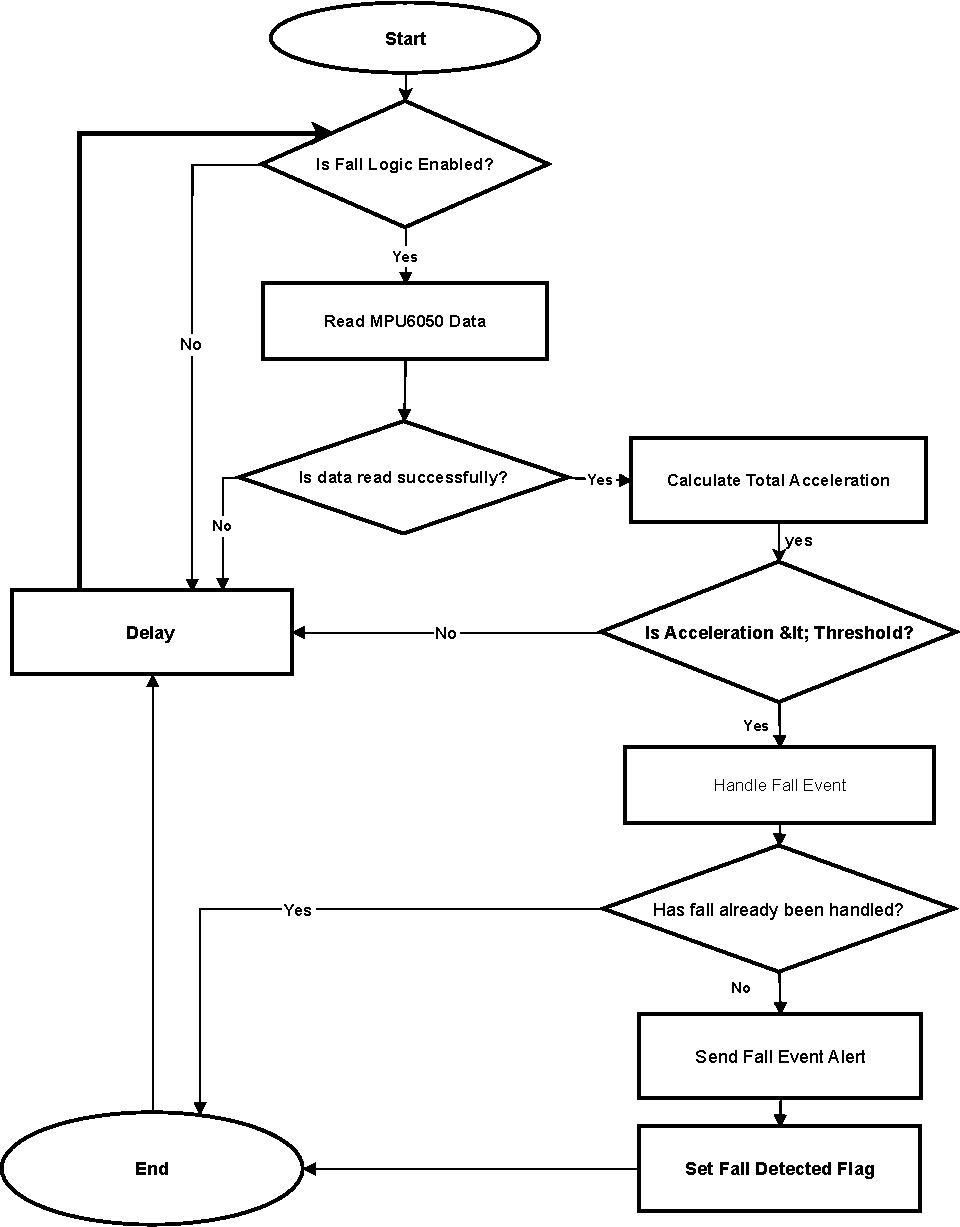
\includegraphics[width=0.85\textwidth,height=0.7\textheight,keepaspectratio]{images/module1_fall_logic_diagram.pdf}
        \caption{Lưu đồ thuật toán phát hiện té ngã.}
        \label{fig:fall_logic_flow}
    \end{figure}
\end{frame}

% Slide: Tổng quan phần mềm Module camera
\begin{frame}{Module camera: Tổng quan phần mềm}
    \begin{block}{Tổng quan}
        \begin{itemize}
            \item Triển khai trên vi điều khiển \textbf{ESP32-S3}.
            \item Thu thập và truyền tải video từ camera \textbf{OV5640} theo thời gian thực.
            \item Cung cấp luồng video MJPEG qua HTTP cho các module xử lý thị giác máy tính.
            \item Dựa trên kiến trúc hướng sự kiện của \textbf{ESP-IDF}, quản lý đồng thời mạng, camera, và bộ đệm.
        \end{itemize}
    \end{block}
    \label{sec:module_ii_software}
\end{frame}

% Slide: Luồng hoạt động chính
\begin{frame}[fragile]{Module camera: Luồng hoạt động chính}
    \begin{block}{Quy trình}
        \begin{enumerate}
            \item \textbf{Khởi tạo hệ thống}: Cấu hình Wi-Fi, camera, và máy chủ HTTP.
            \item \textbf{Chờ yêu cầu client}: Lắng nghe yêu cầu xem video.
            \item \textbf{Lấy khung hình}: Sử dụng triple buffering trên PSRAM để giảm độ trễ.
            \item \textbf{Gửi frame qua HTTP}: Frame JPEG đóng gói trong phản hồi HTTP multipart.
            \item \textbf{Giám sát và xử lý lỗi}: Kiểm tra FPS, xử lý ngắt kết nối client.
        \end{enumerate}
    \end{block}
\end{frame}

% Slide: Sơ đồ luồng hoạt động
\begin{frame}[fragile]{Module camera: Sơ đồ luồng hoạt động}
    \begin{figure}
        \centering
        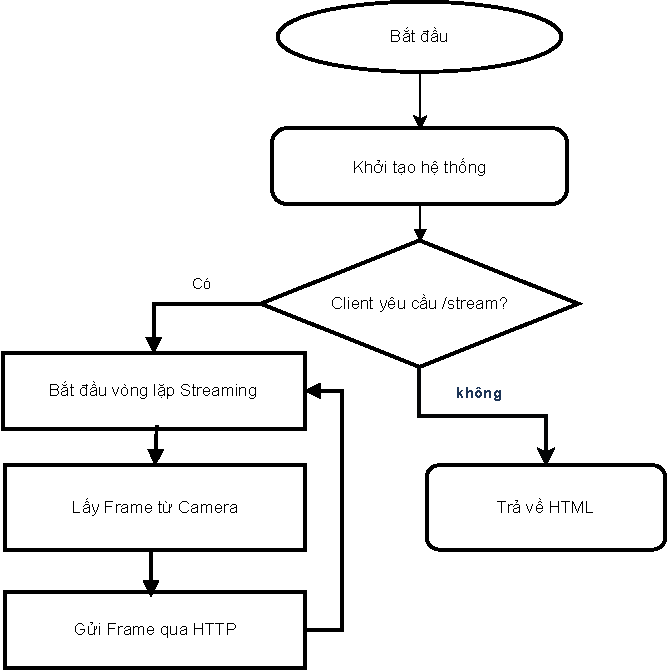
\includegraphics[width=0.85\textwidth,height=0.7\textheight,keepaspectratio]{images/module2_flow_2.pdf}
        \caption{Luồng hoạt động chính của phần mềm Module camera.}
        \label{fig:sw_architecture_flow}
    \end{figure}
\end{frame}

% Slide: Cấu hình phần mềm với Kconfig
\begin{frame}{Module camera: Cấu hình phần mềm với Kconfig}
    \begin{block}{Thông số chính}
        \begin{itemize}
            \item \textbf{Wi-Fi}: SSID và Password để kết nối mạng.
            \item \textbf{Kích thước khung hình}: Từ QQVGA đến UXGA (chất lượng video, băng thông).
            \item \textbf{Chất lượng JPEG}: Giá trị 10–63 (độ nén hình ảnh).
            \item \textbf{Khoảng thời gian giữa các frame}: 0–200 ms (tốc độ khung hình, băng thông).
        \end{itemize}
    \end{block}
\end{frame}

% Slide: Tối ưu hóa hiệu suất và ứng dụng
\begin{frame}{Module camera: Tối ưu hóa hiệu suất và ứng dụng}
    \begin{columns}[t]
        \begin{column}{0.48\textwidth}
            \begin{block}{Kỹ thuật tối ưu}
                \begin{itemize}
                    \item \textbf{Quản lý bộ nhớ}: Sử dụng PSRAM cho buffer, giảm tải SRAM.
                    \item \textbf{Triple buffering}: Chụp frame mới đồng thời với truyền frame cũ.
                    \item \textbf{Giám sát hiệu suất}: Đo FPS thời gian thực, xử lý lỗi ngắt kết nối.
                \end{itemize}
            \end{block}
        \end{column}
        \begin{column}{0.48\textwidth}
            \begin{block}{Ứng dụng}
                \begin{itemize}
                    \item Cầu nối giữa phần cứng và các module xử lý
                    \item Đầu ra video HTTP cho thuật toán thị giác máy tính.
                \end{itemize}
            \end{block}
        \end{column}
    \end{columns}
\end{frame}

\begin{frame}{07_server}
  % TODO: Add content for 07_server
\end{frame}

\begin{frame}{08\_method\_summary}
  % TODO: Add content for 08_method_summary
\end{frame}


% --- Results ---
\section{Kết quả và thực nghiệm}
\subsection{Thiết lập điều kiện thực nghiệm}
\begin{frame}{01\_setup}
    SETUP
\end{frame}
\begin{frame}{Thiết Lập Thực Nghiệm}
\begin{columns}[T]
\begin{column}{0.48\textwidth}

\vspace{0.3cm}
\textbf{Môi trường thử nghiệm:}
\begin{itemize}
\item Trong nhà, điều kiện lý tưởng
\item \textcolor{blue}{Độ chính xác}: Phát hiện đúng té ngã
\item \textcolor{blue}{Độ trễ}: Thời gian cảnh báo
\item \textcolor{blue}{Độ ổn định}: Vận hành liên tục
\end{itemize}
\end{column}

\begin{column}{0.52\textwidth}
\textbf{Cấu hình hệ thống:}
\begin{table}[h!]
\centering
\footnotesize
\begin{tabular}{|p{2.5cm}|p{4cm}|}
\hline
\textbf{Thành phần} & \textbf{Thông số} \\
\hline
Máy chủ & Intel i7-2630QM, GT 525M, Linux Mint \\
\hline
Phần mềm & Asterisk 22.4, Python 3.10.13 \\
\hline
Cảm biến đeo & ESP32 + SIM, Wi-Fi/GSM \\
\hline
Camera & ESP32-S3 + webcam dự phong \\
\hline
Di động & Smartphone + Linphone 6.0.17 \\
\hline
\end{tabular}
\end{table}
\end{column}
\end{columns}

\end{frame}

\subsection{Kiểm thử từng thành phần}

\begin{frame}[t,fragile]
\frametitle{Kiểm thử Module 4G/GPS \& Khởi tạo hệ thống}
\begin{columns}[T]
    %----------------- Column Log -----------------%
    \column{0.55\textwidth}
    \begin{minted}[fontsize=\scriptsize,breaklines]{text}
I (2329)  SIM_4G: Received: Quectel EG800K
OK
I (5329)  SIM_4G: Received: +CSQ: 31,99
OK
I (28339) SIM_4G: Received: +QIACT: 1,1,1,"9.204.251.200"
OK
I (34349) SIM_4G: Received: +QGPSLOC: 10.88862,106.77975
OK
I (9961)  SIM4G_AT: Initializing SIM4G AT driver...
I (10011) APP_MAIN: System initialization complete.
I (10021) APP_MAIN: Application started successfully
    \end{minted}

    %----------------- Column Phân tích -----------------%
    \column{0.45\textwidth}
    \begin{itemize}
        \item \textbf{Mục đích:} 
        \begin{itemize}
            \item Xác nhận giao tiếp AT command, kết nối 4G và thu nhận GPS.
            \item Kiểm tra các module SIM4G-GPS, Wi-Fi và các tác vụ chính.
        \end{itemize}
        \item \textbf{Quy trình:}
        \begin{enumerate}
            \item Khởi tạo UART, kiểm tra modem và SIM.
            \item Đánh giá chất lượng sóng (\texttt{+CSQ}).
            \item Cấu hình APN, kích hoạt PDP context.
            \item Bật GPS và truy vấn tọa độ.
        \end{enumerate}
        \item \textbf{Kết luận:} 
        \begin{itemize}
            \item Module 4G/GPS hoạt động ổn định, sẵn sàng gửi cảnh báo và thông tin định vị.
            \item Hệ thống khởi tạo thành công, tích hợp phần mềm và phần cứng ổn định.
        \end{itemize}
    \end{itemize}
\end{columns}
\end{frame}
% ----------------------------
% Slide: Kiểm thử MQTT
% ----------------------------
\begin{frame}[t,fragile]
\frametitle{Kiểm thử MQTT và truyền dữ liệu}
\begin{columns}[T]
    \column{0.55\textwidth}
    \begin{itemize}
        \item \textbf{Mục đích:} Kiểm tra kết nối broker MQTT và gửi bản tin định kỳ.
        \item \textbf{Log tiêu biểu:}
        \begin{minted}[fontsize=\footnotesize,breaklines]{text}
I (19961) USER_MQTT: MQTT_EVENT_CONNECTED
I (39991) JSON_WRAPPER: {"device_id":"ESP32_DEV_76E48B","fall_detected":false,...}
        \end{minted}
        \item \textbf{Kết luận:} Kết nối MQTT ổn định, dữ liệu được truyền tới hệ thống giám sát.
    \end{itemize}
    \column{0.45\textwidth}
    \begin{figure}
        \centering
        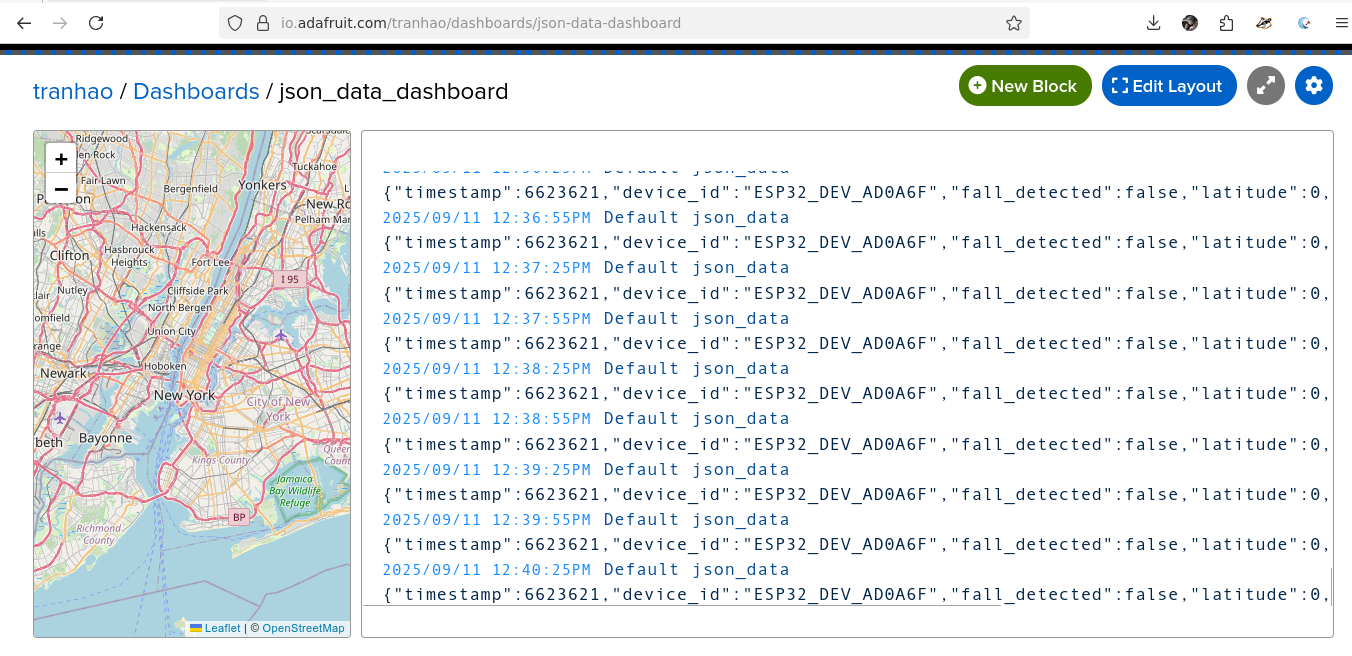
\includegraphics[width=0.75\linewidth]{json_data_dashboard.png}
        \caption{Dashboard hiển thị bản tin MQTT.}
    \end{figure}
\end{columns}
\end{frame}

% ----------------------------
% Slide: Phát hiện té ngã & cảnh báo
% ----------------------------
\begin{frame}[t,fragile]
\frametitle{Phát hiện Té ngã \& Xử lý Cảnh báo}
\begin{columns}[T]
    \column{0.55\textwidth}
    \begin{itemize}
        \item \textbf{Quy trình:}
        \begin{enumerate}
            \item Thuật toán ghi nhận chuỗi trạng thái \texttt{LOW\_G} $\to$ \texttt{HIGH\_G}.
            \item Kích hoạt cảnh báo: SMS, MQTT, buzzer, LED.
        \end{enumerate}
        \item \textbf{Log thực tế:}
        \begin{minted}[fontsize=\footnotesize,breaklines]{text}
\alert{E (159131) FALL_LOGIC: FALL DETECTED! Accel: 0.99 g}
I (159151) SIM4G_GPS: SMS request queued successfully
I (159881) SIM4G_AT: SMS sent successfully.
        \end{minted}
        \item \textbf{Kết luận:} Hệ thống phát hiện và xử lý cảnh báo thành công, đa kênh.
    \end{itemize}
    \column{0.45\textwidth}
    \begin{figure}
        \centering
        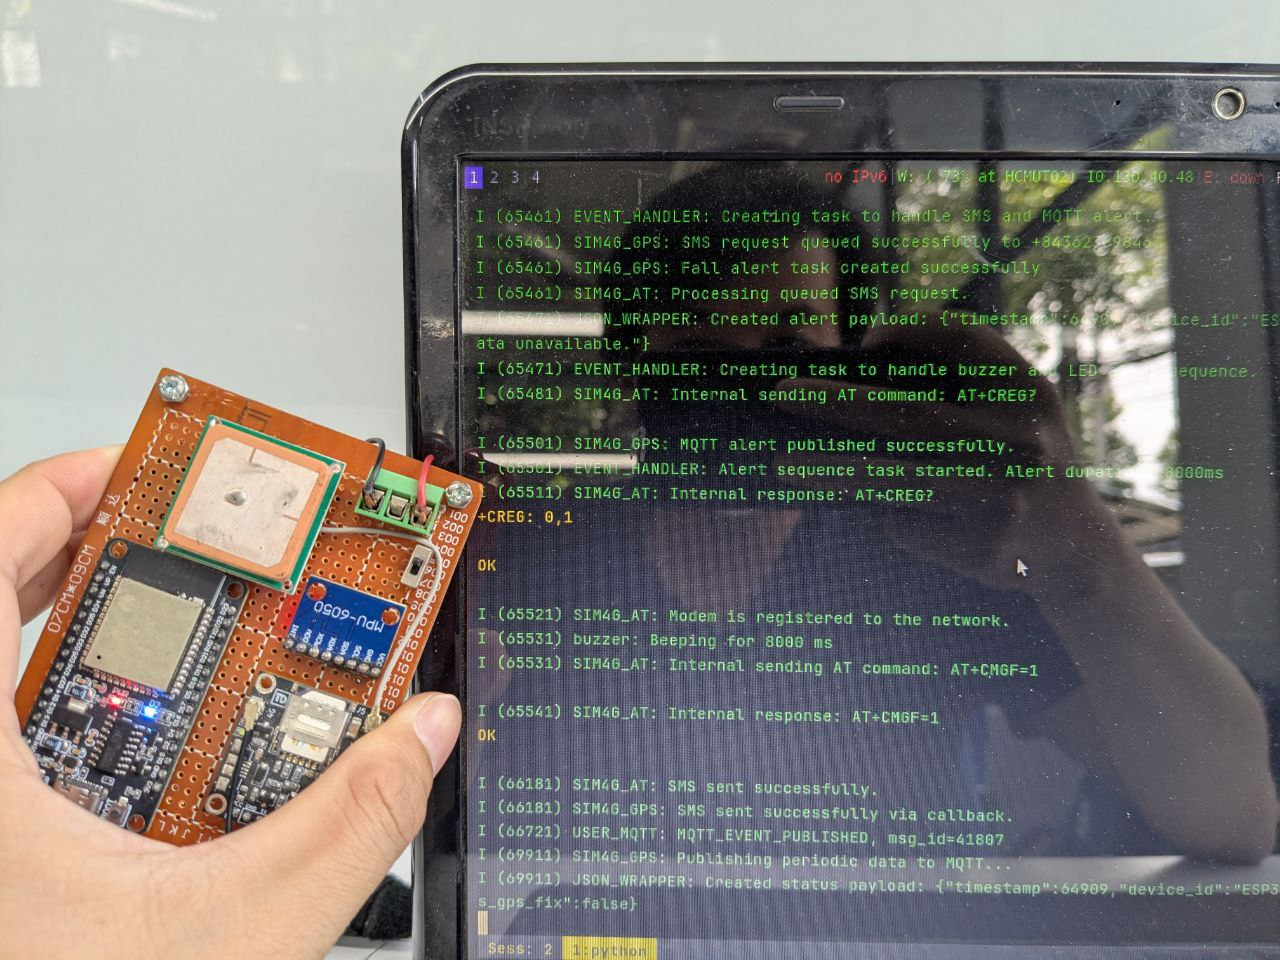
\includegraphics[width=0.75\linewidth]{module1_real_log.jpg}
        \caption{Log thực tế module cảm biến khi phát hiện té ngã.}
    \end{figure}
\end{columns}
\end{frame}

% ----------------------------
% Slide: Camera ESP32 – Luồng hình ảnh & nhận diện
% ----------------------------
\begin{frame}[t,fragile]
\frametitle{Camera ESP32-CAM: Luồng hình ảnh và xử lý}
\begin{columns}[T]
    %----------------- Column Hình -----------------%
    \column{0.55\textwidth}
    \begin{figure}[H]
        \centering
        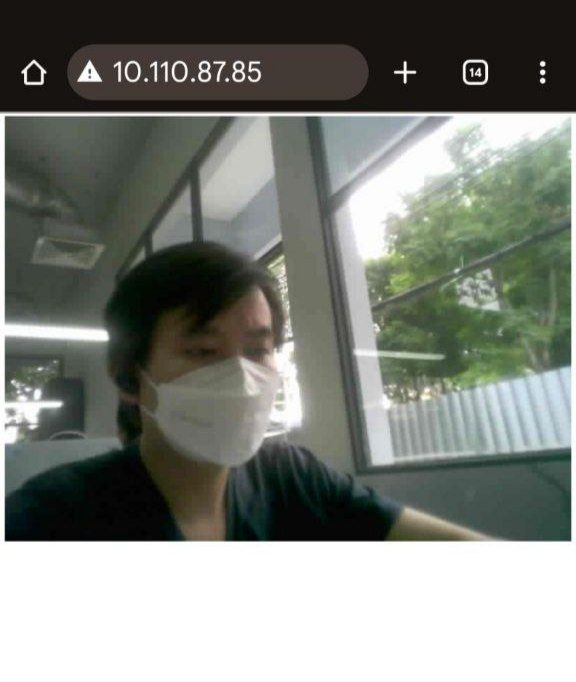
\includegraphics[width=\linewidth]{module2_stream_example.jpg}
        \caption{Luồng hình ảnh từ ESP32-CAM qua HTTP.}
    \end{figure}

    %----------------- Column Phân tích -----------------%
    \column{0.45\textwidth}
    \begin{itemize}
        \item \textbf{Mục đích:} Kiểm tra kết nối Wi-Fi và phát luồng hình ảnh.
        \item \textbf{Xử lý Python:}
        \begin{itemize}
            \item Nhận luồng video từ ESP32-CAM.
            \item Tiền xử lý khung hình.
            \item TensorFlow Lite phát hiện người, vẽ skeleton.
        \end{itemize}
        \item \textbf{Kết quả:} Thời gian thực 3–5 FPS, hoạt động ổn định.
        \item \textbf{Ứng dụng:} Cảnh báo té ngã, đồng bộ MQTT, gửi thông báo Telegram.
    \end{itemize}
\end{columns}
\end{frame}

% ----------------------------
% Slide: Xử lý nhận diện hình ảnh (Python)
% ----------------------------
\begin{frame}[t]
\frametitle{Xử lý nhận diện hình ảnh (Python)}
\begin{itemize}
    \item \textbf{Mục đích:} Phát hiện người và trích xuất skeleton từ luồng video.
    \item \textbf{Quy trình:}
    \begin{itemize}
        \item Nhận luồng video từ ESP32-CAM.
        \item Tiền xử lý khung hình.
        \item TensorFlow Lite phát hiện người, vẽ skeleton.
    \end{itemize}
    \item \textbf{Kết quả:} Thời gian thực 3–5 FPS, hoạt động ổn định.
\end{itemize}
\end{frame}

% ----------------------------
% Slide: Kết quả xử lý hình ảnh
% ----------------------------
\begin{frame}[t]
\frametitle{Kết quả xử lý hình ảnh}
\begin{figure}
    \centering
    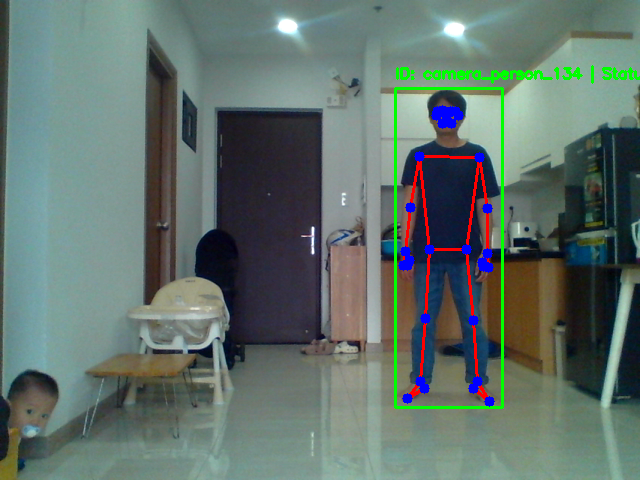
\includegraphics[width=0.75\linewidth]{fall_detection_screen_shoot.png}
    \caption{Module Python phát hiện người và vẽ skeleton.}
\end{figure}
\end{frame}

% ----------------------------
% Slide: Log thực nghiệm Python
% ----------------------------
\begin{frame}[fragile]
\frametitle{Log thực nghiệm Python}
\begin{figure}[H]
    \centering
    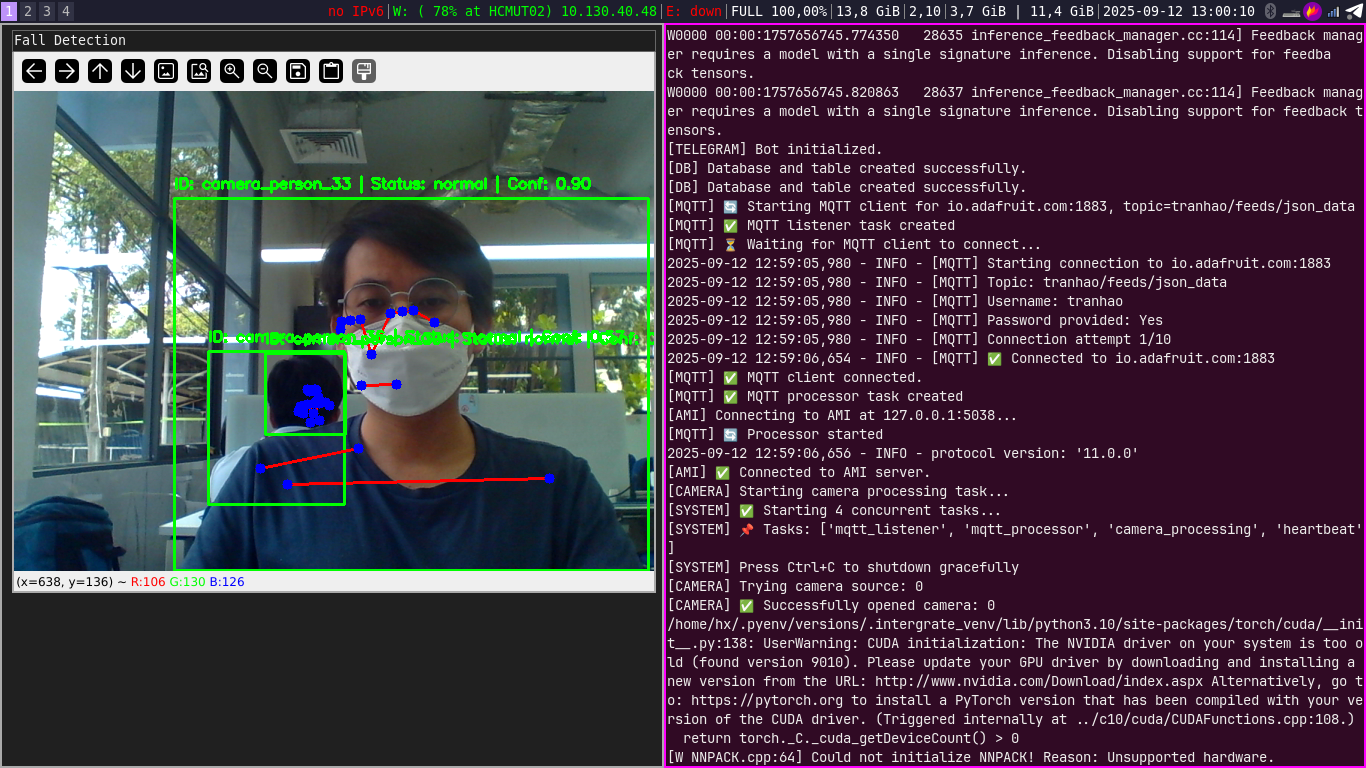
\includegraphics[width=0.75\linewidth]{python_runing_log.png}
    \caption{Log Python xử lý luồng camera và cảnh báo.}
\end{figure}
\begin{itemize}
    \item \textbf{Kết luận:} Module Python hoạt động ổn định, đồng bộ MQTT và kích hoạt cảnh báo thành công.
\end{itemize}
\end{frame}

% ----------------------------
% Slide: Đánh giá dữ liệu cảm biến MPU6050
% ----------------------------
\begin{frame}[fragile]
\frametitle{Đánh giá dữ liệu cảm biến (MPU6050)}
\begin{itemize}
    \item \textbf{Quy trình:} Giả lập té ngã, so sánh dữ liệu bình thường và té ngã.
    \item \textbf{Kết quả:}
    \begin{itemize}
        \item \textbf{Gyro (dps):} Bình thường $\approx \pm 1.5$; té ngã tăng $\approx \pm 250$.
        \item \textbf{Accel (g):} Bình thường $\approx 0.93$; té ngã $-2.0$ đến $+1.0$.
    \end{itemize}
    \item \textbf{Kết luận:} \textbf{Accel\_Mag} và \textbf{Gyro\_Mag} là chỉ báo hiệu quả.
\end{itemize}
\end{frame}

% ----------------------------
% Slide: Biến thiên Gyro_Mag
% ----------------------------

\begin{frame}[t,fragile]
\frametitle{Biến thiên & Phân tích Gyro\_Mag}
\begin{columns}[T]
    \column{0.55\textwidth}
    \begin{figure}[H]
        \centering
        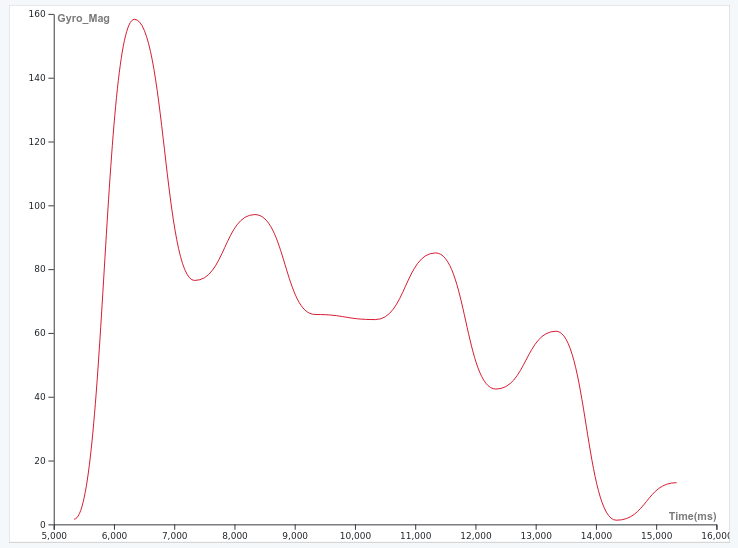
\includegraphics[width=\linewidth]{gyro_time.png}
        \caption{Magnitude gia tốc góc theo thời gian. Peak biểu thị té ngã.}
    \end{figure}
    \column{0.45\textwidth}
    \begin{itemize}
        \item \textbf{Bình thường:} Dao động nhỏ ($\lesssim 2$ dps).
        \item \textbf{Sự kiện té ngã:} Xuất hiện đỉnh lớn (hàng chục–trăm dps).
        \item \textbf{Hậu té:} Giảm nhanh về mức nền, trạng thái nằm yên.
    \end{itemize}
\end{columns}
\end{frame}
% ----------------------------
% Slide: Biến thiên Accel_Mag

\begin{frame}[t,fragile]
\frametitle{Biến thiên & Phân tích Accel\_Mag}
\begin{columns}[T]
    %----------------- Column Hình -----------------%
    \column{0.55\textwidth}
    \begin{figure}[H]
        \centering
        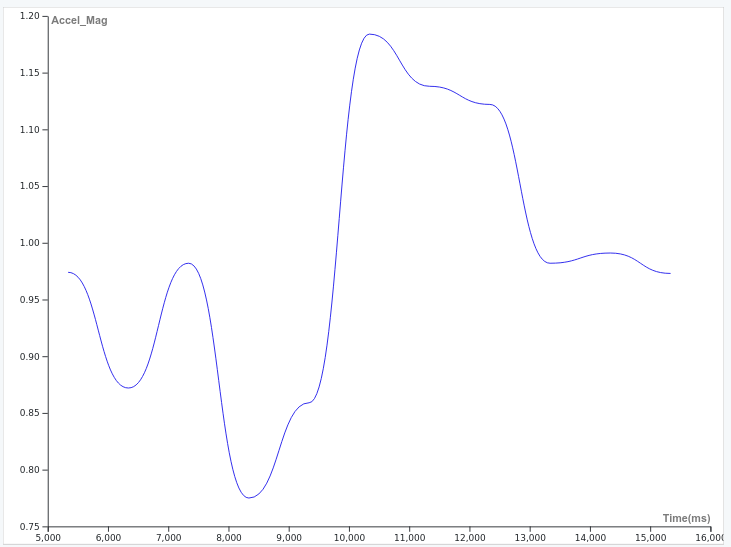
\includegraphics[width=\linewidth]{accel_time.png}
        \caption{Magnitude gia tốc (Accel\_Mag) theo thời gian. Xung lớn biểu thị té ngã.}
    \end{figure}
    %----------------- Column Phân tích -----------------%
    \column{0.45\textwidth}
    \begin{itemize}
        \item \textbf{Bình thường:} Gần 1\,g, dao động nhỏ.
        \item \textbf{Sự kiện té ngã:} Xuất hiện xung hoặc thay đổi đột ngột, vượt hoặc giảm mạnh so với 1\,g.
        \item \textbf{Hậu té:} Trở về gần 1\,g nhưng phân bố vector khác (tư thế nằm).
    \end{itemize}
\end{columns}
\end{frame}
% ----------------------------
% Slide: Kiểm thử cảnh báo Asterisk AMI
% ----------------------------
\begin{frame}[fragile]
\frametitle{Kiểm thử cảnh báo qua Asterisk AMI}
\begin{itemize}
    \item \textbf{Mục đích:} Kiểm chứng cuộc gọi và SMS tự động.
    \item \textbf{Kết quả:}
    \begin{itemize}
        \item Kết nối thành công tới Asterisk AMI.
        \item SMS tới \texttt{6001, 6002} thành công; \texttt{6003} lỗi.
        \item Lỗi gọi điện không ảnh hưởng đến cảnh báo chính.
    \end{itemize}
\end{itemize}
\begin{figure}[H]
    \centering
    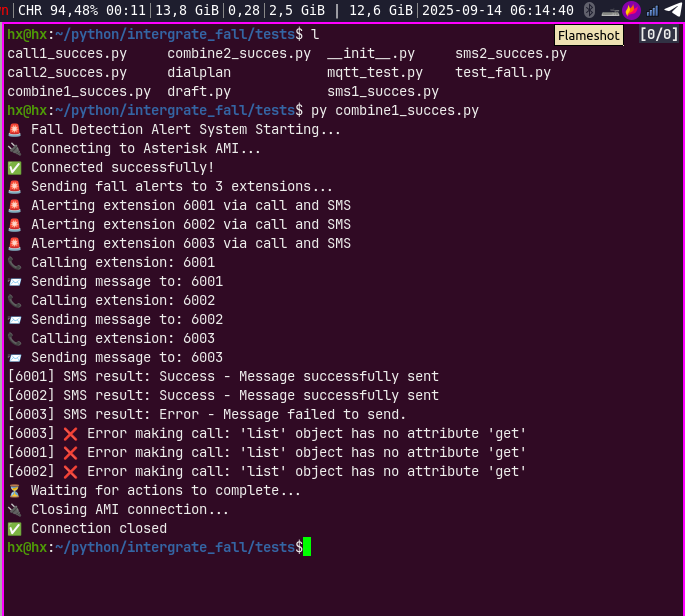
\includegraphics[width=0.75\linewidth]{ast_call_sms_test.png}
    \caption{Thử nghiệm chức năng gọi và nhắn tin.}
\end{figure}
\end{frame}

% ----------------------------
% Slide: Kiểm thử cảnh báo Telegram
% ----------------------------
\begin{frame}[t,fragile]
\frametitle{Kiểm thử cảnh báo qua Telegram}
\begin{itemize}
    \item \textbf{Cơ chế hoạt động:}
    \begin{itemize}
        \item \textbf{Phần cứng:} MQTT từ thiết bị -> trung tâm -> Telegram.
        \item \textbf{Python:} Camera -> Python gửi cảnh báo trực tiếp Telegram kèm hình.
    \end{itemize}
\end{itemize}
\end{frame}

% ----------------------------
% Slide: Thông báo Telegram
% ----------------------------
\begin{frame}[t,fragile]
\frametitle{Thông báo Telegram}
\begin{columns}[T]
    \column{0.5\textwidth}
    \begin{figure}[H]
        \centering
        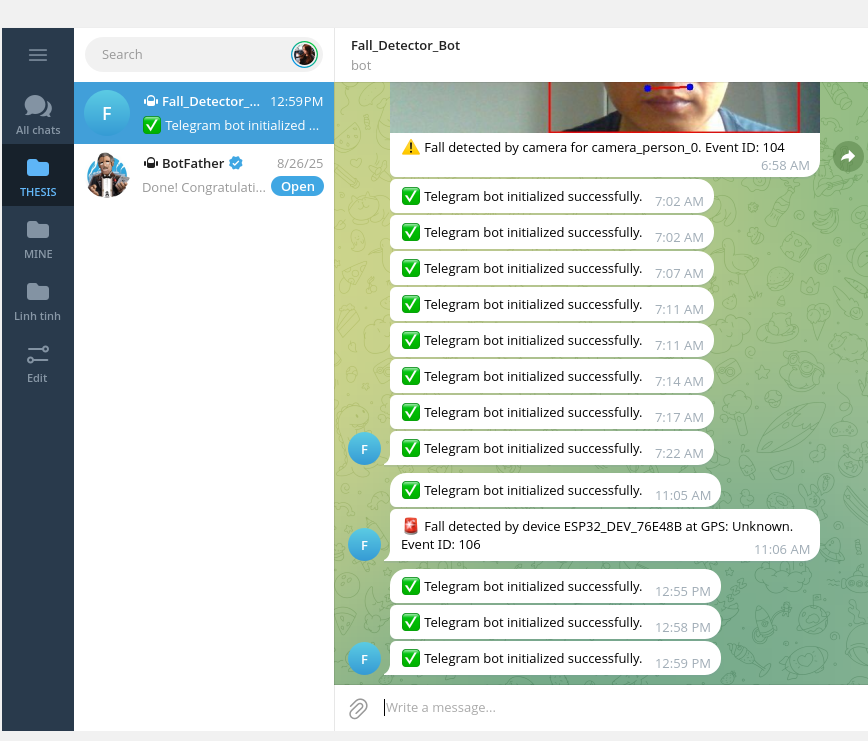
\includegraphics[width=0.75\linewidth]{telegram_fall_module1_send.png}
        \caption{Thông báo từ phần cứng.}
    \end{figure}
    \column{0.5\textwidth}
    \begin{figure}[H]
        \centering
        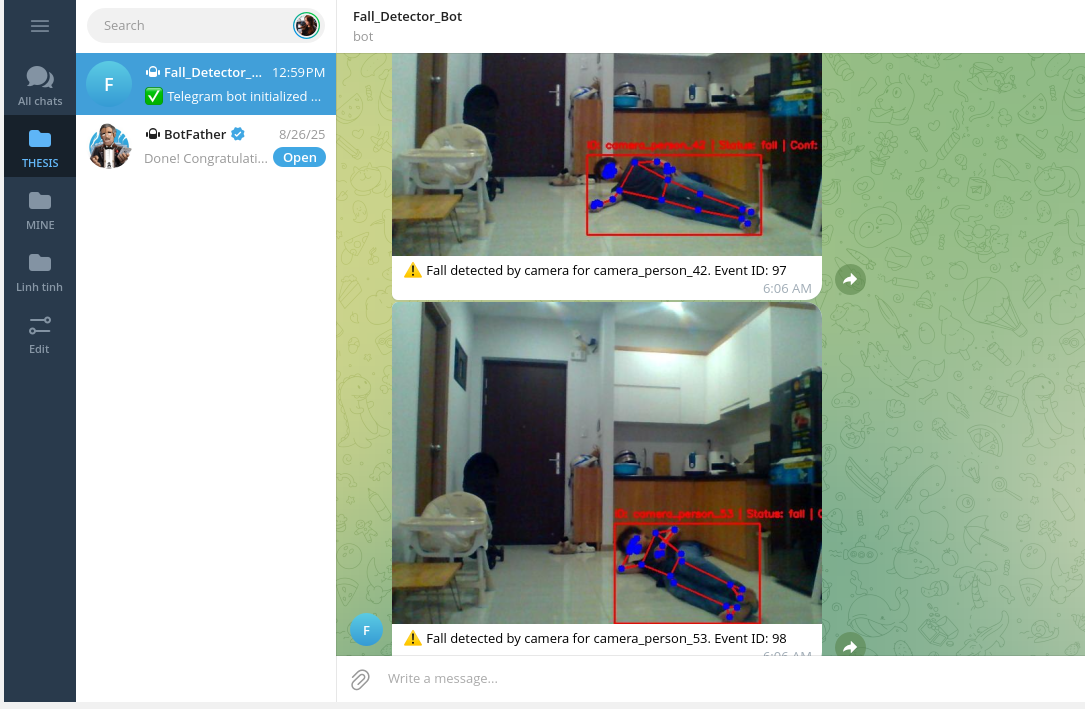
\includegraphics[width=0.75\linewidth]{telegram_python_fall_send.png}
        \caption{Thông báo từ Python.}
    \end{figure}
    \vspace{2mm}
    \begin{itemize}
        \item \textbf{Kết luận:} Kênh Telegram hoạt động ổn định, đa nguồn cảnh báo tăng độ tin cậy.
    \end{itemize}
\end{columns}
\end{frame}

%
\begin{frame}{Phân tích độ trễ & Đánh giá độ ổn định}
\begin{columns}[T]
    %---------------- Column 1: Độ trễ ----------------%
    \column{0.55\textwidth}
    \textbf{Độ trễ hệ thống (Latency)}
    \begin{tabular}{@{}ll@{}}
    \toprule
    \textbf{Khâu} & \textbf{Mô tả} \\
    \midrule
    ESP32 & Đọc cảm biến, xử lý phát hiện té ngã, phát cảnh báo \\
    Mạng & Truyền gói MQTT tới broker \\
    Dịch vụ & Python nhận dữ liệu, kích hoạt bot Telegram \\
    \bottomrule
    \end{tabular}

    %---------------- Column 2: Đánh giá độ ổn định ----------------%
    \column{0.45\textwidth}
    \textbf{Đánh giá độ ổn định}
    \begin{itemize}
        \item Thiết bị hoạt động liên tục, không tràn bộ nhớ, không reset đột ngột.
        \item Phần mềm Python chạy ổn định, xử lý ngoại lệ tốt, dữ liệu phối hợp chính xác.
        \item Giật/lag khung hình do giới hạn phần cứng, không ảnh hưởng tổng thể.
        \item Hệ thống đạt độ ổn định cao trong điều kiện thử nghiệm liên tục.
    \end{itemize}
\end{columns}
\end{frame}

%\begin{frame}{04_stability}
  % TODO: Add content for 04_stability
\end{frame}

\begin{frame}{Đánh giá kết quả thực nghiệm}
\begin{columns}[T]
    %---------------- Column 1: Độ trễ ----------------%
    \column{0.5\textwidth}
    \textbf{Độ trễ hệ thống (Latency)}
    \begin{itemize}
        \item \textbf{ESP32}: đọc cảm biến, xử lý và phát cảnh báo.
        \item \textbf{Mạng}: truyền gói MQTT tới broker.
        \item \textbf{Dịch vụ}: Python nhận dữ liệu, kích hoạt bot Telegram.
        \item \textbf{Tổng thể}: độ trễ < 5 giây, đáp ứng gần thời gian thực.
    \end{itemize}

    %---------------- Column 2: Đánh giá độ ổn định ----------------%
    \column{0.5\textwidth}
    \textbf{Đánh giá độ ổn định \& hiệu năng}
    \begin{itemize}
        \item Hệ thống hoạt động liên tục, không tràn bộ nhớ hay reset đột ngột.
        \item Thuật toán phân biệt rõ trạng thái bình thường và té ngã.
        \item Dữ liệu phối hợp chính xác, phần mềm Python ổn định.
        \item Giật/lag do phần cứng, không ảnh hưởng tổng thể.
    \end{itemize}
\end{columns}
\end{frame}



% --- Conclusion ---
\section{V-KẾT LUẬN}
\begin{frame}{01_summary}
  % TODO: Add content for 01_summary
\end{frame}

%\begin{frame}{02_contribution}
  % TODO: Add content for 02_contribution
\end{frame}

%\begin{frame}{03_limitations}
  % TODO: Add content for 03_limitations
\end{frame}

%\begin{frame}{04_futurework}
  % TODO: Add content for 04_futurework
\end{frame}

%\begin{frame}{05_overall}
  % TODO: Add content for 05_overall
\end{frame}


% --- Thank you ---
%\begin{frame}{01_thankyou}
  % TODO: Add content for 01_thankyou
\end{frame}


% ========================
% Kết thúc tài liệu
% ========================
\end{document}

